\documentclass[11pt,addpoints,answers]{exam}

%%%%%%%%%%%%%%%%%%%%%%%%%%%%%%%%%%%%%%%%%%%
% Commands for customizing the assignment %
%%%%%%%%%%%%%%%%%%%%%%%%%%%%%%%%%%%%%%%%%%%
\newcommand{\hwNum}{Homework 7}
\newcommand{\hwTopic}{Deep Learning}
\newcommand{\hwName}{\hwNum: \hwTopic}
\newcommand{\outDate}{Thusrday, Nov 7th}
\newcommand{\dueDate}{Sunday, Nov 17th}
\newcommand{\taNames}{Bhargav, Maxwell, Sebastian, Varsha, Zachary, Neural the Narwhal}
\newcommand{\homeworktype}{\string written, programming}

\newcommand{\summary}{
    \begin{notebox}
        \paragraph{Summary} In this assignment you will implement an RNN and performance evaluation. You will begin by going through some conceptual questions about CNNs, RNNs, and transformers for intuition for deep learning models and then use that intuition to build your own models.
    \end{notebox}
}
%% To HIDE SOLUTIONS (to post at the website for students), set this value to 0: \def\issoln{0}
\providecommand{\issoln}{0}
% \providecommand{\issoln}{1}

 %-----------------------------------------------------------------------------
% PACKAGES AND OTHER DOCUMENT CONFIGURATIONS
%-----------------------------------------------------------------------------

\usepackage[margin=1in]{geometry}
\usepackage{bbm}
\usepackage{amsmath, amsfonts}
\usepackage{enumerate}
\usepackage{graphicx}
\usepackage{titling}
\usepackage{url}
\usepackage{xfrac}
\usepackage{natbib}
\usepackage{amssymb}
\usepackage{amsthm}
\usepackage{paralist}
\usepackage{epstopdf}
\usepackage{tabularx}
\usepackage{longtable}
\usepackage{multirow}
\usepackage{multicol}
\usepackage[colorlinks=true,urlcolor=blue]{hyperref}
\usepackage{algorithm}
\usepackage{algorithmicx}
\usepackage[noend]{algpseudocode}
\usepackage{float}
\usepackage{enumerate}
\usepackage{array}
\usepackage{environ}
\usepackage{times}
\usepackage{textcomp}
\usepackage{caption}
\usepackage{parskip} % For NIPS style paragraphs.
\usepackage[compact]{titlesec} % Less whitespace around titles
\usepackage[inline]{enumitem} % For inline enumerate* and itemize*
\usepackage{datetime}
\usepackage{comment}
% \usepackage{minted}
\usepackage{lastpage}
\usepackage{color}
\usepackage{xcolor}
\usepackage[final]{listings}
\usepackage{framed}
\usepackage{booktabs}
\usepackage{cprotect}
\usepackage{verbatim}
\usepackage{verbatimbox}
\usepackage{multicol}
\usepackage{hyperref}
\usepackage{subcaption}
\usepackage{mathtools} % For drcases
\usepackage{cancel}
\usepackage[many]{tcolorbox}
\usepackage{soul}
\usepackage[bottom]{footmisc}
\usepackage{bm}
\usepackage{wasysym}
\usepackage{pgfplots}
\usepackage{tikz}
\usetikzlibrary{shapes,decorations,arrows}
\usetikzlibrary{arrows.meta}
\usetikzlibrary{shapes.geometric}
\usetikzlibrary{positioning, arrows, automata, calc}
\usepackage{transparent}
\usepackage{tikz-cd}


\newtcolorbox[]{your_solution}[1][]{
    % breakable,
    enhanced,
    nobeforeafter,
    colback=white,
    title=Your Answer,
    sidebyside align=top,
    box align=top,
    #1
}


%%%%%%%%%%%%%%%%%%%%%%%%%%%%%%%%%%%%%%%%%%%
% Rotated Column Headers                  %
%%%%%%%%%%%%%%%%%%%%%%%%%%%%%%%%%%%%%%%%%%%
\usepackage{adjustbox}
\usepackage{array}

%https://tex.stackexchange.com/questions/32683/rotated-column-titles-in-tabular

\newcolumntype{R}[2]{%
    >{\adjustbox{angle=#1,lap=\width-(#2)}\bgroup}%
    l%
    <{\egroup}%
}
\newcommand*\rot{\multicolumn{1}{R{45}{1em}}}% no optional argument here, please!


%%%%%%%%%%%%%%%%%%%%%%%%%%%%%%%%%%%%%%%%%%%
% Formatting for \CorrectChoice of "exam" %
%%%%%%%%%%%%%%%%%%%%%%%%%%%%%%%%%%%%%%%%%%%

\CorrectChoiceEmphasis{}
\checkedchar{\blackcircle}

\newenvironment{checkboxessquare}{
    \begingroup
    \checkboxchar{$\Box$} \checkedchar{$\blacksquare$} % change checkbox style locally
    \begin{checkboxes}
    }{
    \end{checkboxes}
    \endgroup
    }

%%%%%%%%%%%%%%%%%%%%%%%%%%%%%%%%%%%%%%%%%%%
% Better numbering                        %
%%%%%%%%%%%%%%%%%%%%%%%%%%%%%%%%%%%%%%%%%%%

% \numberwithin{equation}{section} % Number equations within sections (i.e. 1.1, 1.2, 2.1, 2.2 instead of 1, 2, 3, 4)
% \numberwithin{figure}{section} % Number figures within sections (i.e. 1.1, 1.2, 2.1, 2.2 instead of 1, 2, 3, 4)
% \numberwithin{table}{section} % Number tables within sections (i.e. 1.1, 1.2, 2.1, 2.2 instead of 1, 2, 3, 4)

%%%%%%%%%%%%%%%%%%%%%%%%%%%%%%%%%%%%%%%%%%
% Custom commands                        %
%%%%%%%%%%%%%%%%%%%%%%%%%%%%%%%%%%%%%%%%%%
\newcommand{\R}{\mathbb{R}}
\newcommand{\blackcircle}{\tikz\draw[black,fill=black] (0,0) circle (1ex);}
\renewcommand{\circle}{\tikz\draw[black] (0,0) circle (1ex);}


%%%%%%%%%%%%%%%%%%%%%%%%%%%%%%%%%%%%%%%%%%
% Custom commands for Math               %
%%%%%%%%%%%%%%%%%%%%%%%%%%%%%%%%%%%%%%%%%%
\newcommand{\vc}[1]{\boldsymbol{#1}}
\newcommand{\adj}[1]{\frac{\partial \ell}{\partial #1}}
\newcommand{\chain}[2]{\adj{#2} = \adj{#1}\frac{\partial #1}{\partial #2}}
\newcommand{\ntset}{test}
\newcommand{\zerov}{\mathbf{0}}
\DeclareMathOperator*{\argmin}{argmin}

% mathcal
\newcommand{\Ac}{\mathcal{A}}
\newcommand{\Bc}{\mathcal{B}}
\newcommand{\Cc}{\mathcal{C}}
\newcommand{\Dc}{\mathcal{D}}
\newcommand{\Ec}{\mathcal{E}}
\newcommand{\Fc}{\mathcal{F}}
\newcommand{\Gc}{\mathcal{G}}
\newcommand{\Hc}{\mathcal{H}}
\newcommand{\Ic}{\mathcal{I}}
\newcommand{\Jc}{\mathcal{J}}
\newcommand{\Kc}{\mathcal{K}}
\newcommand{\Lc}{\mathcal{L}}
\newcommand{\Mc}{\mathcal{M}}
\newcommand{\Nc}{\mathcal{N}}
\newcommand{\Oc}{\mathcal{O}}
\newcommand{\Pc}{\mathcal{P}}
\newcommand{\Qc}{\mathcal{Q}}
\newcommand{\Rc}{\mathcal{R}}
\newcommand{\Sc}{\mathcal{S}}
\newcommand{\Tc}{\mathcal{T}}
\newcommand{\Uc}{\mathcal{U}}
\newcommand{\Vc}{\mathcal{V}}
\newcommand{\Wc}{\mathcal{W}}
\newcommand{\Xc}{\mathcal{X}}
\newcommand{\Yc}{\mathcal{Y}}
\newcommand{\Zc}{\mathcal{Z}}

% mathbb
\newcommand{\Ab}{\mathbb{A}}
\newcommand{\Bb}{\mathbb{B}}
\newcommand{\Cb}{\mathbb{C}}
\newcommand{\Db}{\mathbb{D}}
\newcommand{\Eb}{\mathbb{E}}
\newcommand{\Fb}{\mathbb{F}}
\newcommand{\Gb}{\mathbb{G}}
\newcommand{\Hb}{\mathbb{H}}
\newcommand{\Ib}{\mathbb{I}}
\newcommand{\Jb}{\mathbb{J}}
\newcommand{\Kb}{\mathbb{K}}
\newcommand{\Lb}{\mathbb{L}}
\newcommand{\Mb}{\mathbb{M}}
\newcommand{\Nb}{\mathbb{N}}
\newcommand{\Ob}{\mathbb{O}}
\newcommand{\Pb}{\mathbb{P}}
\newcommand{\Qb}{\mathbb{Q}}
\newcommand{\Rb}{\mathbb{R}}
\newcommand{\Sb}{\mathbb{S}}
\newcommand{\Tb}{\mathbb{T}}
\newcommand{\Ub}{\mathbb{U}}
\newcommand{\Vb}{\mathbb{V}}
\newcommand{\Wb}{\mathbb{W}}
\newcommand{\Xb}{\mathbb{X}}
\newcommand{\Yb}{\mathbb{Y}}
\newcommand{\Zb}{\mathbb{Z}}

% mathbf lowercase
\newcommand{\av}{\mathbf{a}}
\newcommand{\bv}{\mathbf{b}}
\newcommand{\cv}{\mathbf{c}}
\newcommand{\dv}{\mathbf{d}}
\newcommand{\ev}{\mathbf{e}}
\newcommand{\fv}{\mathbf{f}}
\newcommand{\gv}{\mathbf{g}}
\newcommand{\hv}{\mathbf{h}}
\newcommand{\iv}{\mathbf{i}}
\newcommand{\jv}{\mathbf{j}}
\newcommand{\kv}{\mathbf{k}}
\newcommand{\lv}{\mathbf{l}}
\newcommand{\mv}{\mathbf{m}}
\newcommand{\nv}{\mathbf{n}}
\newcommand{\ov}{\mathbf{o}}
\newcommand{\pv}{\mathbf{p}}
\newcommand{\qv}{\mathbf{q}}
\newcommand{\rv}{\mathbf{r}}
\newcommand{\sv}{\mathbf{s}}
\newcommand{\tv}{\mathbf{t}}
\newcommand{\uv}{\mathbf{u}}
\newcommand{\vv}{\mathbf{v}}
\newcommand{\wv}{\mathbf{w}}
\newcommand{\xv}{\mathbf{x}}
\newcommand{\yv}{\mathbf{y}}
\newcommand{\zv}{\mathbf{z}}

% mathbf uppercase
\newcommand{\Av}{\mathbf{A}}
\newcommand{\Bv}{\mathbf{B}}
\newcommand{\Cv}{\mathbf{C}}
\newcommand{\Dv}{\mathbf{D}}
\newcommand{\Ev}{\mathbf{E}}
\newcommand{\Fv}{\mathbf{F}}
\newcommand{\Gv}{\mathbf{G}}
\newcommand{\Hv}{\mathbf{H}}
\newcommand{\Iv}{\mathbf{I}}
\newcommand{\Jv}{\mathbf{J}}
\newcommand{\Kv}{\mathbf{K}}
\newcommand{\Lv}{\mathbf{L}}
\newcommand{\Mv}{\mathbf{M}}
\newcommand{\Nv}{\mathbf{N}}
\newcommand{\Ov}{\mathbf{O}}
\newcommand{\Pv}{\mathbf{P}}
\newcommand{\Qv}{\mathbf{Q}}
\newcommand{\Rv}{\mathbf{R}}
\newcommand{\Sv}{\mathbf{S}}
\newcommand{\Tv}{\mathbf{T}}
\newcommand{\Uv}{\mathbf{U}}
\newcommand{\Vv}{\mathbf{V}}
\newcommand{\Wv}{\mathbf{W}}
\newcommand{\Xv}{\mathbf{X}}
\newcommand{\Yv}{\mathbf{Y}}
\newcommand{\Zv}{\mathbf{Z}}

% bold greek lowercase
\newcommand{\alphav     }{\boldsymbol \alpha     }
\newcommand{\betav      }{\boldsymbol \beta      }
\newcommand{\gammav     }{\boldsymbol \gamma     }
\newcommand{\deltav     }{\boldsymbol \delta     }
\newcommand{\epsilonv   }{\boldsymbol \epsilon   }
\newcommand{\varepsilonv}{\boldsymbol \varepsilon}
\newcommand{\zetav      }{\boldsymbol \zeta      }
\newcommand{\etav       }{\boldsymbol \eta       }
\newcommand{\thetav     }{\boldsymbol \theta     }
\newcommand{\varthetav  }{\boldsymbol \vartheta  }
\newcommand{\iotav      }{\boldsymbol \iota      }
\newcommand{\kappav     }{\boldsymbol \kappa     }
\newcommand{\varkappav  }{\boldsymbol \varkappa  }
\newcommand{\lambdav    }{\boldsymbol \lambda    }
\newcommand{\muv        }{\boldsymbol \mu        }
\newcommand{\nuv        }{\boldsymbol \nu        }
\newcommand{\xiv        }{\boldsymbol \xi        }
\newcommand{\omicronv   }{\boldsymbol \omicron   }
\newcommand{\piv        }{\boldsymbol \pi        }
\newcommand{\varpiv     }{\boldsymbol \varpi     }
\newcommand{\rhov       }{\boldsymbol \rho       }
\newcommand{\varrhov    }{\boldsymbol \varrho    }
\newcommand{\sigmav     }{\boldsymbol \sigma     }
\newcommand{\varsigmav  }{\boldsymbol \varsigma  }
\newcommand{\tauv       }{\boldsymbol \tau       }
\newcommand{\upsilonv   }{\boldsymbol \upsilon   }
\newcommand{\phiv       }{\boldsymbol \phi       }
\newcommand{\varphiv    }{\boldsymbol \varphi    }
\newcommand{\chiv       }{\boldsymbol \chi       }
\newcommand{\psiv       }{\boldsymbol \psi       }
\newcommand{\omegav     }{\boldsymbol \omega     }

% bold greek uppercase
\newcommand{\Gammav     }{\boldsymbol \Gamma     }
\newcommand{\Deltav     }{\boldsymbol \Delta     }
\newcommand{\Thetav     }{\boldsymbol \Theta     }
\newcommand{\Lambdav    }{\boldsymbol \Lambda    }
\newcommand{\Xiv        }{\boldsymbol \Xi        }
\newcommand{\Piv        }{\boldsymbol \Pi        }
\newcommand{\Sigmav     }{\boldsymbol \Sigma     }
\newcommand{\Upsilonv   }{\boldsymbol \Upsilon   }
\newcommand{\Phiv       }{\boldsymbol \Phi       }
\newcommand{\Psiv       }{\boldsymbol \Psi       }
\newcommand{\Omegav     }{\boldsymbol \Omega     }

%%%%%%%%%%%%%%%%%%%%%%%%%%%%%%%%%%%%%%%%%%%
% Code highlighting with listings         %
%%%%%%%%%%%%%%%%%%%%%%%%%%%%%%%%%%%%%%%%%%%

\definecolor{bluekeywords}{rgb}{0.13,0.13,1}
\definecolor{greencomments}{rgb}{0,0.5,0}
\definecolor{redstrings}{rgb}{0.9,0,0}
\definecolor{light-gray}{gray}{0.95}

\newcommand{\MYhref}[3][blue]{\href{#2}{\color{#1}{#3}}}%

\definecolor{dkgreen}{rgb}{0,0.6,0}
\definecolor{gray}{rgb}{0.5,0.5,0.5}
\definecolor{mauve}{rgb}{0.58,0,0.82}

\lstdefinelanguage{Shell}{
  keywords={tar, cd, make},
  %keywordstyle=\color{bluekeywords}\bfseries,
  alsoletter={+},
  ndkeywords={python, py, javac, java, gcc, c, g++, cpp, .txt, octave, m, .tar},
  %ndkeywordstyle=\color{bluekeywords}\bfseries,
  identifierstyle=\color{black},
  sensitive=false,
  comment=[l]{//},
  morecomment=[s]{/*}{*/},
  commentstyle=\color{purple}\ttfamily,
  %stringstyle=\color{red}\ttfamily,
  morestring=[b]',
  morestring=[b]",
  backgroundcolor = \color{light-gray}
}

\lstset{columns=fixed, basicstyle=\ttfamily,
    backgroundcolor=\color{light-gray},xleftmargin=0.5cm,frame=tlbr,framesep=4pt,framerule=0pt}

\newcommand{\emptysquare}{{\LARGE $\square$}\ \ }
\newcommand{\filledsquare}{{\LARGE $\boxtimes$}\ \ }
\def \ifempty#1{\def\temp{#1} \ifx\temp\empty }

\def \squaresolutionspace#1{ \ifempty{#1} \emptysquare \else #1\hspace{0.75pt}\fi}

\newcommand{\emptycircle}{{\LARGE $\fullmoon$}\ \ }
\newcommand{\filledcircle}{{\LARGE $\newmoon$}\ \ }
\def \circlesolutionspace#1{ \ifempty{#1} \emptycircle \else #1\hspace{0.75pt}\fi}

%%%%%%%%%%%%%%%%%%%%%%%%%%%%%%%%%%%%%%%%%%%
% Custom box for highlights               %
%%%%%%%%%%%%%%%%%%%%%%%%%%%%%%%%%%%%%%%%%%%

% Define box and box title style
\tikzstyle{mybox} = [fill=blue!10, very thick,
    rectangle, rounded corners, inner sep=1em, inner ysep=1em]

% \newcommand{\notebox}[1]{
% \begin{tikzpicture}
% \node [mybox] (box){%
%     \begin{minipage}{\textwidth}
%     #1
%     \end{minipage}
% };
% \end{tikzpicture}%
% }

\NewEnviron{notebox}{

\begin{tikzpicture}
\node [mybox] (box){
    \begin{minipage}{\textwidth}
        \BODY
    \end{minipage}
};
\end{tikzpicture}
}

%%%%%%%%%%%%%%%%%%%%%%%%%%%%%%%%%%%%%%%%%%%
% Commands showing / hiding solutions     %
%%%%%%%%%%%%%%%%%%%%%%%%%%%%%%%%%%%%%%%%%%%

%%%%%%%%%%%%%%%%%%%%%%%%%%%%%%%%%%%%%%%%%%%
% Commands showing / hiding solutions     %
%%%%%%%%%%%%%%%%%%%%%%%%%%%%%%%%%%%%%%%%%%%
\newcommand{\solutionspace}[4]{\fbox{\begin{minipage}[t][#1][t]{#2} \textbf{#3} \solution{}{#4} \end{minipage}}}

%% To HIDE SOLUTIONS (to post at the website for students), set this value to 0: \def\issoln{0}
% \def\issoln{0} % Uncomment to remove solutions
% \def\issoln{1} % Uncomment to show solutions

% Some commands to allow solutions to be embedded in the assignment file.
\ifcsname issoln\endcsname \else \def\issoln{1} \fi

% Default to an empty solutions environ.
\NewEnviron{soln}{}{}
\if\issoln 1

% Otherwise, include solutions as below.
 \RenewEnviron{soln}{
    \leavevmode\color{red}\ignorespaces   %textbf{Solution} \BODY
    \BODY
 }{}
\fi

%%%%%%%%%%%%%%%%

%% qauthor environment:
% Default to an empty qauthor environ.
\NewEnviron{qauthor}{}{}

%% To HIDE TAGS set this value to 0:
\def\showtags{0}  % Uncomment to remove tags
% \def\showtags{1} % Uncomment to show tags


\ifcsname showtags\endcsname \else \def\showtags{1} \fi

% Default to an empty tags environ.
\NewEnviron{tags}{}{}
\if\showtags 1

% Otherwise, include solutions as below.
\RenewEnviron{tags}{
    \fbox{
    \leavevmode\color{blue}\ignorespaces
    \textbf{TAGS:} \texttt{\url{\BODY}}
    }
    \vspace{-.5em}
}{}
\fi

% Default to an empty learning objective environment
\NewEnviron{qlearningobjective}{}
%%%%%%%%%%%%%%%%%%%%%%%%%%%%%%%%%%%%%%%%%%%%%%%%%
% Useful commands for typesetting the questions %
%%%%%%%%%%%%%%%%%%%%%%%%%%%%%%%%%%%%%%%%%%%%%%%%%

\newcommand \expect {\mathbb{E}}
\newcommand \mle [1]{{\hat #1}^{\rm MLE}}
\newcommand \map [1]{{\hat #1}^{\rm MAP}}
\newcommand \argmax {\operatorname*{argmax}}
% \newcommand \argmin {\operatorname*{argmin}}
\newcommand \code [1]{{\tt #1}}
\newcommand \datacount [1]{\#\{#1\}}
\newcommand \ind [1]{\mathbb{I}\{#1\}}

%%%%%%%%%%%%%%%%%%%%%%%%%%
% Document configuration %
%%%%%%%%%%%%%%%%%%%%%%%%%%

% Don't display a date in the title and remove the white space
\predate{}
\postdate{}
\date{}

% Don't display an author and remove the white space
%\preauthor{}
%\postauthor{}

% Solo and group questions
\newcommand{\solo}{\textbf{[SOLO]} }
\newcommand{\group}{\textbf{[GROUP]} }

% Question type commands
\newcommand{\sall}{\textbf{Select all that apply: }}
\newcommand{\sone}{\textbf{Select one: }}
\newcommand{\tf}{\textbf{True or False: }}

% AdaBoost commands
\newcommand{\trainerr}[1]{\hat{\epsilon}_S \left(#1\right)}
\newcommand{\generr}[1]{\epsilon \left(#1\right)}
\newcommand{\D}{\mathcal{D}}
\newcommand{\margin}{\text{margin}}
\newcommand{\sign}{\text{sign}}
\newcommand{\PrS}{\hat{\Pr_{(x_i, y_i) \sim S}}}
\newcommand{\PrSinline}{\hat{\Pr}_{(x_i, y_i) \sim S}}  % inline PrS

% Abhi messing around with examdoc
\qformat{\textbf{{\Large \thequestion \; \; \thequestiontitle \ (\totalpoints \ points)}} \hfill}
\renewcommand{\thequestion}{\arabic{question}}
\renewcommand{\questionlabel}{\thequestion.}

\renewcommand{\thepartno}{\arabic{partno}}
\renewcommand{\partlabel}{\thepartno.}
\renewcommand{\partshook}{\setlength{\leftmargin}{0pt}}

\renewcommand{\thesubpart}{\alph{subpart}}
\renewcommand{\subpartlabel}{(\thesubpart)}

\renewcommand{\thesubsubpart}{\roman{subsubpart}}
\renewcommand{\subsubpartlabel}{\thesubsubpart.}

% copied from stack overflow, as all good things are
\newcommand\invisiblesection[1]{%
  \refstepcounter{section}%
  \addcontentsline{toc}{section}{\protect\numberline{\thesection}#1}%
  \sectionmark{#1}}

% quite possibly the worst workaround i have made for this class
\newcommand{\sectionquestion}[1]{
\titledquestion{#1}
\invisiblesection{#1}
~\vspace{-1em}
}

% also copied from stack overflow
% https://tex.stackexchange.com/questions/153846/indent-every-subsubsection-element
% and edited following
% https://latexref.xyz/bs-at-startsection.html
% PLEASE DELETE THIS FOR OTHER HOMEWORK
% \ifnum\pdfstrcmp{\taNames}{Sana, Chu, Hayden, Tori, Prasoon}=0
% \makeatletter
% \newcommand\subsectionquestion{%
%   \@startsection{subsection}{2}
%   {-2pc}% <------- The opposite of what we set for subs
%   {-3.25ex\@plus -1ex \@minus -.2ex}%
%   {1.5ex \@plus .2ex}%
%   {\normalfont\large\bfseries}}
% \makeatother
% \fi

%%%%%%%%%%%%%%%%%%%%%%%%%%%%%%%%%%%%%%%%%%%
% New Environment for Pseudocode          %
%%%%%%%%%%%%%%%%%%%%%%%%%%%%%%%%%%%%%%%%%%%

% Python style for highlighting
\DeclareFixedFont{\ttb}{T1}{txtt}{bx}{n}{12} % for bold
\DeclareFixedFont{\ttm}{T1}{txtt}{m}{n}{12}  % for normal

\definecolor{deepblue}{rgb}{0,0,0.5}
\definecolor{deepred}{rgb}{0.6,0,0}
\definecolor{deepgreen}{rgb}{0,0.5,0}

\newcommand\pythonstyle{\lstset{
language=Python,
basicstyle=\ttm,
morekeywords={self},              % Add keywords here
keywordstyle=\ttb\color{deepblue},
emph={MyClass,__init__},          % Custom highlighting
emphstyle=\ttb\color{deepred},    % Custom highlighting style
stringstyle=\color{deepgreen},
frame=tb,                         % Any extra options here
showstringspaces=false
}}


% Python environment
\lstnewenvironment{your_code_solution}[1][]
{
\pythonstyle
\lstset{#1}
}
{}
\newtcolorbox[]{your_code_solution_outer}[1][]{
    % breakable,
    enhanced,
    nobeforeafter,
    colback=white,
    title=Your Answer,
    sidebyside align=top,
    box align=top,
    #1
}
%%%%%%%%%%%%%%%%%%%%%%%%%%%%%%%%%%%%%%%%%%%
% Commands for customizing the assignment %
%%%%%%%%%%%%%%%%%%%%%%%%%%%%%%%%%%%%%%%%%%%
\newcommand{\courseNum}{10-301 / 10-601}
\newcommand{\courseName}{Introduction to Machine Learning}
\newcommand{\courseSem}{Fall 2024}
\newcommand{\courseUrl}{\url{http://www.cs.cmu.edu/~mgormley/courses/10601/}}

%\pagestyle{fancyplain}
\lhead{\hwName}
\rhead{\courseNum}
\cfoot{\thepage{} of \numpages{}}

\title{\textsc{\hwNum}: \textsc{\hwTopic} 
\thanks{Compiled on \today{} at \currenttime{}} \\
\vspace{1em}
} % Title

\author{\textsc{\large \courseNum{} \courseName{} (\courseSem)}\\
\courseUrl
\vspace{1em}\\
  OUT: \outDate \\
  DUE: \dueDate \\
  TAs: \taNames\\
}

\date{}
\begin{document}
\maketitle
\summary{}
\section*{START HERE: Instructions}
\begin{itemize}
\newcommand \maxsubs {10 }

\item \textbf{Collaboration Policy}: Please read the collaboration policy here: \url{http://www.cs.cmu.edu/~mgormley/courses/10601/syllabus.html}

\item\textbf{Late Submission Policy:} See the late submission policy here: \url{http://www.cs.cmu.edu/~mgormley/courses/10601/syllabus.html}

\item\textbf{Submitting your work:} You will use Gradescope to submit
  answers to all questions\ifthenelse{\equal{\homeworktype}{\string written}}{}{ and code}. Please
  follow instructions at the end of this PDF to correctly submit all your code to Gradescope.

\begin{itemize}
    
    \item \textbf{Written:} For written problems such as short answer, multiple choice, derivations, proofs, or plots, please use the provided template. Submissions can be handwritten onto the template, but should be labeled and clearly legible. If your writing is not legible, you will not be awarded marks. Alternatively, submissions can be written in \LaTeX{}. Each derivation/proof should be completed in the boxes provided. You are responsible for ensuring that your submission contains exactly the same number of pages and the same alignment as our PDF template. If you do not follow the template, your assignment may not be graded correctly by our AI assisted grader and there will be a \textbf{\textcolor{red}{2\% penalty}} (e.g., if the homework is out of 100 points, 2 points will be deducted from your final score).
    %
    % This policy is NOT in effect when we have the Background Test.
    % \ifthenelse{\equal{\homeworktype}{\string hw1}}{ {\color{red} For this assignment only, if you answer at least 90\% of the written questions correctly, you get full marks on the written portion of this assignment. For this assignment only, \textbf{we will offer two rounds of grading}. The first round of grading will happen immediately following the due date specified above. We will then release your grades to you and if you got less than 90\% on the written questions, you will be allowed to submit once again by a second due date. The exact due date for the second round will be announced after we release the first round grades. } }{}

    \ifthenelse{\equal{\homeworktype}{\string written}}{}{
    \item \textbf{Programming:} You will submit your code for programming questions on the homework to \href{https://gradescope.com}{Gradescope}. After uploading your code, our grading scripts will autograde your assignment by running your program on a virtual machine (VM). 
    %
    You are only permitted to use \href{https://docs.python.org/3/library/}{the Python Standard Library modules} and \texttt{numpy}.
    % You are only permitted to use \href{https://docs.python.org/3/library/}{the Python Standard Library modules}, \texttt{numpy} and the modules already imported in the starter notebook. You are not permitted to import any other modules.
    %
    % You will not have to change the default version of your programming environment and the versions of the permitted libraries on Google Colab. You have \maxsubs free Gradescope programming submissions, after which you will begin to lose points from your total programming score. We recommend debugging your implementation on Google Colab and making sure your code is running correctly first before submitting your code to Gradescope.}
    %
    Ensure that the version number of your programming language environment (i.e. Python 3.9.12) and versions of permitted libraries (i.e. \texttt{numpy} 1.23.0) match those used on Gradescope. You have \maxsubs free Gradescope programming submissions, after which you will begin to lose points from your total programming score. We recommend debugging your implementation on your local machine (or the Linux servers) and making sure your code is running correctly first before submitting your code to Gradescope.}
    \ifthenelse{\equal{\homeworktype}{\string hw1}}{ {\color{red} The submission limit is true for future assignments, but this one allows \textbf{unlimited submissions.}} }{}
   
  \end{itemize}
  
\ifthenelse{\equal{\homeworktype}{\string written}}{}{\item\textbf{Materials:} The data and reference output that you will need in order to complete this assignment is posted along with the writeup and template on the course website.}

\end{itemize}

\section*{Instructions for Specific Problem Types}

For ``Select One" questions, please fill in the appropriate bubble completely:

\begin{quote}
\textbf{Select One:} Who taught this course?
    \begin{checkboxes}
     \CorrectChoice Matt Gormley
     \choice Marie Curie
     \choice Noam Chomsky
    \end{checkboxes}
\end{quote}

If you need to change your answer, you may cross out the previous answer and bubble in the new answer:

\begin{quote}
\textbf{Select One:} Who taught this course?
    {
    \begin{checkboxes}
     \CorrectChoice Henry Chai
     \choice Marie Curie \checkboxchar{\xcancel{\blackcircle}{}}
     \choice Noam Chomsky
    \end{checkboxes}
    }
\end{quote}

For ``Select all that apply" questions, please fill in all appropriate squares completely:

\begin{quote}
\textbf{Select all that apply:} Which are instructors for this course?
    {%
    \checkboxchar{$\Box$} \checkedchar{$\blacksquare$} % change checkbox style locally
    \begin{checkboxes}
    \CorrectChoice Matt Gormley  
    \CorrectChoice Henry Chai
    \choice Noam Chomsky
    \choice I don't know
    \end{checkboxes}
    }
\end{quote}

Again, if you need to change your answer, you may cross out the previous answer(s) and bubble in the new answer(s):

\begin{quote}
\textbf{Select all that apply:} Which are the instructors for this course?
    {%
    \checkboxchar{\xcancel{$\blacksquare$}} \checkedchar{$\blacksquare$} % change checkbox style locally
    \begin{checkboxes}
    \CorrectChoice Matt Gormley 
    \CorrectChoice Henry Chai
    \choice Noam Chomsky
    \choice I don't know
    \end{checkboxes}
    }
\end{quote}

For questions where you must fill in a blank, please make sure your final answer is fully included in the given space. You may cross out answers or parts of answers, but the final answer must still be within the given space.

\begin{quote}
\textbf{Fill in the blank:} What is the course number?

\begin{tcolorbox}[fit,height=1cm, width=4cm, blank, borderline={1pt}{-2pt},nobeforeafter]
    \begin{center}\huge10-601\end{center}
    \end{tcolorbox}\hspace{2cm}
    \begin{tcolorbox}[fit,height=1cm, width=4cm, blank, borderline={1pt}{-2pt},nobeforeafter]
    \begin{center}\huge10-\xcancel{6}301\end{center}
    \end{tcolorbox}
\end{quote}

\clearpage
{\LARGE \bf Written Questions (\numpoints \ points)} 
\begin{questions}
\sectionquestion{\LaTeX{} Point and Template Alignment}
\begin{parts}
    \part[1] \sone Did you use \LaTeX{} for the entire written portion of this homework?
    
    \begin{checkboxes}
        % YOUR ANSWER
        % Change \choice to \CorrectChoice for the appropriate selection/selections 
        \CorrectChoice Yes 
        \choice No
    \end{checkboxes}

    \part[0] \sone I have ensured that my final submission is aligned with the original template given to me in the handout file and that I haven't deleted or resized any items or made any other modifications which will result in a misaligned template. I understand that incorrectly responding yes to this question will result in a penalty equivalent to 2\% of the points on this assignment.\\
    \textbf{Note:} Failing to answer this question will not exempt you from the 2\% misalignment penalty.
    
    \begin{checkboxes}
        % YOUR ANSWER
        % Change \choice to \CorrectChoice for the appropriate selection/selections 
        \CorrectChoice Yes 
    \end{checkboxes}
\end{parts}
\sectionquestion{Convolutional Neural Network}
\label{sec:cnn}
\begin{parts}

\part In this problem, consider a convolutional layer from a standard implementation of a CNN as described in lecture, without any bias term. 

\begin{figure}[h]
    \centering
    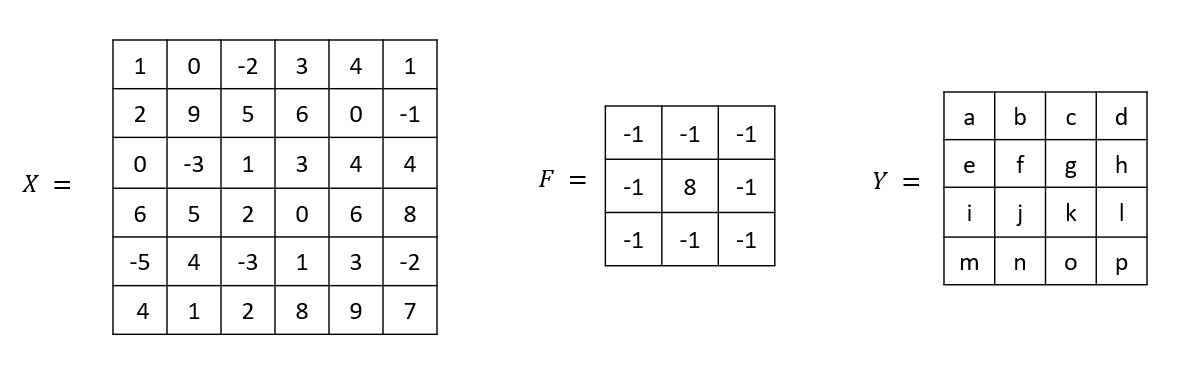
\includegraphics[scale=0.6]{figs/CNN.PNG}
\end{figure}
    \begin{subparts}
    \subpart[1] Let an image $X$ $(6\times6)$ be convolved with a filter $F$ $(3\times3)$ using no padding and a stride of $1$ to produce an output $Y$  $(4\times4$). What is value of $j$ in the output $Y$?\\
    \begin{your_solution}[height=2cm,width=4cm]
    % YOUR ANSWER 
    8
    \end{your_solution}
    
    \vspace{4mm}
    
    \subpart[1] Suppose you instead had an input feature map (or image) of size $6 \times 4$ (height $\times$ width) and a filter of size $2 \times 2$, using no padding and a stride of $2$, what would be the resulting output size? Write your answer in the format: height $\times$ width.\\
    \begin{your_solution}[height=2cm,width=4cm]
    % YOUR ANSWER 
    3x2
    \end{your_solution} 
    \end{subparts}


% \break

\part Parameter sharing is a very important concept for CNN  because it drastically reduces the complexity of the learning problem and consequently that of the model required to tackle it. The following questions will deal with parameter sharing. Assume that there is no bias term in our convolutional layer.

\begin{subparts}
    \subpart[1] \sall Which of the following are parameters of a convolutional layer?
    \checkboxchar{$\Box$} \checkedchar{$\blacksquare$}
    \begin{checkboxes}
        % YOUR ANSWER 
        % Change \choice to \CorrectChoice for the appropriate selection
        \choice Stride size
        \choice Padding size
        \choice Input size
        \choice Filter size
        \CorrectChoice Weights in the filter
        \choice None of the above
    \end{checkboxes}
    
    \vspace{4mm}
    
    \subpart[1] \sall Which of the following are hyperparameters of a convolutional layer?
    \checkboxchar{$\Box$} \checkedchar{$\blacksquare$}
    \begin{checkboxes}
        % YOUR ANSWER 
        % Change \choice to \CorrectChoice for the appropriate selection
        \CorrectChoice Stride size
        \CorrectChoice Padding size
        \CorrectChoice Input size
        \CorrectChoice Filter size
        \choice Weights in the filter
        \choice None of the above
    \end{checkboxes}
    
    \vspace{4mm}

    \subpart[1] Suppose for the convolutional layer, we are given grayscale images of size $22\times 22$. Using one single $4 \times 4$ filter with a stride of $2$, no padding and a single output channel, what is the \textbf{number of parameters} you are learning in this layer? \\
    \begin{your_solution}[height=2cm,width=4cm]
        % YOUR ANSWER 
        16
    \end{your_solution}\\
    
    \vspace{4mm}
    
    \subpart[1] Now suppose we do not do parameter sharing. That is, each output pixel of this layer is computed by a separate $4 \times 4$ filter. Again we use a stride of $2$, no padding and a single output channel. What is the \textbf{number of parameters} you are learning in this layer? \\
    \begin{your_solution}[height=2cm,width=4cm]
        % YOUR ANSWER 
        1600
    \end{your_solution}

    \newpage
    
    \subpart[1] Now suppose you are given a $40 \times 40$ colored image, which consists of $3$ channels, each representing the intensity of one primary color (so your input is a $40 \times 40 \times 3$ tensor). Once again, you attempt to produce an output map without parameter sharing, using a unique $4 \times 4$ filter per output pixel, with a stride of $2$, no padding and a single output channel (so the number of channels in the filter are the same as the number of channels in the input image). What is the number of parameters you are learning in this layer? \\
    \begin{your_solution}[height=2cm,width=4cm]
        % YOUR ANSWER 
        17328
    \end{your_solution}\\

    \vspace{4mm}

    \subpart[1] In \textit{one concise sentence}, describe a reason why parameter sharing is a good idea for a convolutional layer applied to image data, besides the reduction in number of learned parameters.  \\
    \begin{your_solution}[height=5cm]
        % YOUR ANSWER
        Parameter sharing helps to find similar patterns among different locations in an image, making the feature detection through convolution layer reaches spatially invariant.
    \end{your_solution}\\
\end{subparts}

\vspace{4mm}

\part Neural the Narwhal was expecting to implement a CNN for Homework 5, but he is disappointed that he only got to write a simple fully-connected neural network. 
\begin{subparts}

\subpart[2] Neural decides to implement a CNN himself and comes up with the following naive implementation:
\begin{lstlisting}[language=Python,escapechar=@]
# image X has shape (H_in, W_in), and filter F has shape (K, K)
# the output Y has shape (H_out, W_out)
Y = np.zeros((H_out, W_out))
for r in range(H_out):
    for c in range(W_out):
        for i in range(K):
            for j in range(K):
                Y[r, c] += X[@\underline{$~~~\emph{\texttt{blank}}~~~$}@] * F[i, j]
\end{lstlisting}
What should be in the \textit{blank} above so that the output \texttt{Y} is correct? Assume that \texttt{H\_out} and \texttt{W\_out} are pre-computed correctly, the filter has a stride of 1 and there's no padding. \\
    \begin{your_solution}[height=1.75cm]
    % YOUR ANSWER 
    % Put your solution in the your_code_solution environment
    \begin{your_code_solution}
    	r+i, c+j
    \end{your_code_solution}
    
    \end{your_solution}

\newpage

\subpart[2] Neural now wants to implement the backpropagation part of the network but is stuck. He decides to go to office hours to ask for help. One TA tells him that a CNN can actually be implemented using matrix multiplication. He receives the following 1D convolution example:
\begin{quote}
    Suppose you have an input vector $\xv = [x_1, x_2, x_3, x_4, x_5]^T$ and a 1D convolution filter $\wv = [w_1, w_2, w_3]^T$. Then if the output is $\yv = [y_1, y_2, y_3]^T$, $y_1 = w_1 x_1 + w_2 x_2 + w_3 x_3$, $y_2 = \cdots$, $y_3 = \cdots$. If you look at this closely, this is equivalent to
    \[
    \begin{bmatrix} y_1 \\ y_2 \\ y_3 \end{bmatrix} = \Av \begin{bmatrix} x_1 \\ x_2 \\ x_3 \\ x_4 \\ x_5 \end{bmatrix}
    \]
    where the matrix $\Av$ is given as $\cdots$
\end{quote}
What is matrix $\Av$ for this $\xv$, $\yv$ and $\wv$? Write only the final answer. Your work will \textit{not} be graded. \\
    \begin{your_solution}[height=5cm]
        % YOUR ANSWER 
        % Use `bmatrix` to typeset a matrix.
        % Example:
        % \[
        % \begin{bmatrix}
        % 1 & 2 & 3 \\
        % 4 & 5 & 6
        % \end{bmatrix}
        % \]
        % is a 2 x 3 matrix where the first row has elements 1, 2, 3 and the first column has elements 1, 4.
        % Make sure you put the bmatrix in something like \[ ... \] or in $ ... $
    
    $A = \begin{bmatrix}
	w_1 & w_2 & w_3 & 0 & 0 \\
	0 & w_1 & w_2 & w_3 & 0 \\
	0 & 0 & w_1 & w_2 & w_3 \\
	\end{bmatrix}$    
    \end{your_solution}

\vspace{5mm}

\subpart[2] Neural wonders why the TA told him about matrix multiplication when he wanted to write the backpropagation part. Then he notices that the gradient is extremely simple with this version of CNN. Explain in \textit{one concise sentence (or one short mathematical expression)} how you can compute $\frac{\partial \yv}{\partial \xv}$ once you obtain $\Av$ for some \textit{arbitrary} input $\xv$, filter $\wv$, and the corresponding 1D convolution output $\yv$ (so $\Av$ is obtained following the same procedure as in part (b), but $\xv$, $\yv$ and $\wv$ can be different from the example). Write only the final answer. Your work will \textit{not} be graded. \\
    \begin{your_solution}[height=2cm]
        % YOUR ANSWER 
    $\frac{\partial \yv}{\partial \xv} = A^{T}$
    
    \end{your_solution}


\end{subparts}

\end{parts}

\newpage    \newpage

\sectionquestion{Recurrent Neural Network}
\label{sec:rnn}
\begin{parts}

\part Consider the following simple RNN architecture:
\begin{center}

\begin{tikzcd}[cells={nodes={draw=gray}}]
	& {\hat{\yv}_1} & {\hat{\yv}_2} & {\hat{\yv}_3} \\
	{\hv_0} & {\hv_1} & {\hv_2} & {\hv_3} \\
	& {\xv_1} & {\xv_2} & {\xv_3}
	\arrow[from=2-1, to=2-2]
	\arrow[from=2-2, to=2-3]
	\arrow[from=2-3, to=2-4]
	\arrow[from=3-4, to=2-4]
	\arrow[from=3-3, to=2-3]
	\arrow[from=3-2, to=2-2]
	\arrow[from=2-2, to=1-2]
	\arrow[from=2-3, to=1-3]
	\arrow[from=2-4, to=1-4]
\end{tikzcd}
\end{center}
where we have inputs $\xv_t$, hidden states $\hv_t$, and outputs $\hat{\yv}_t$ for each timestep $t$. The dimensions of these and the weights of the model are given below. On the right, we show the computation, performed by the RNN to obtain the outputs $\hat{\yv}_t$ and subsequently the loss $J$ for a single input $\xv_{1:3}$. 

\begin{minipage}{0.5\linewidth}
\begin{align*}
    \xv_t &\in \mathbb{R}^3 &\Wv_{hx} &\in \mathbb{R}^{4 \times 3}\\
    \hv_t &\in \mathbb{R}^4 &\Wv_{hy} &\in \mathbb{R}^{2 \times 4}\\
    \yv_t, \hat{\yv}_t &\in \mathbb{R}^2 &\Wv_{hh} &\in \mathbb{R}^{4 \times 4}\\
\end{align*}
\end{minipage}
\begin{minipage}{0.5\linewidth}    
\begin{align*}
    \zv_t &= \Wv_{hh} \hv_{t-1} + \Wv_{hx}\xv_t\\
    \hv_t &= \psi(\zv_t)\\
    \ov_t &= \Wv_{hy}\hv_t\\
    \hat{\yv}_t &= soft(\ov_t)\\
    J_t &= -\sum_{i=1}^2 y_{t,i} \log(\hat{y}_{t,i})\\
    J &= \sum_{t=1}^3 J_t\\
\end{align*}
\end{minipage}

Above $\yv_t$ is a one-hot vector representing the label for the $t$th timestep, $soft$ is the \textbf{softmax} activation, $\psi$ is the \textbf{identity} activation (i.e. no activation), $J$ is the cross entropy loss computed by the function $CE()$. Note here that we assume that we have no intercept term. 

\begin{subparts}

\clearpage
    \subpart[4] You will now construct the unrolled computational graph for the given model.
    Use input sequence $\xv$, label $\yv$, and the RNN equations presented above to complete the graph by filling in the solution boxes for the corresponding blanks.\\

    \begin{center}
    \[\begin{tikzcd}[cells={nodes={draw=gray}}]
	&& {J = \sum_{t=1}^3 J_t} \\
	&& {\Wv_{hy}} \\
	&& {\yv_2} & {\yv_3} \\
	{\yv_1} & {J_1 = CE(\hat{\yv}_{1}, \yv_1)} & {\textbf{part (c)}} & {J_3 = CE(\hat{\yv}_{3}, \yv_3)} \\
	& {\hat{\yv}_1 = soft(\ov_1)} & {\hat{\yv}_2 = soft(\ov_2)} & {\hat{\yv}_3 = soft(\ov_3)} \\
	& {\textbf{part (a)}} & {\ov_2 = Lin(\Wv_{hy}, \hv_2)} & {\ov_3 = Lin(\Wv_{hy}, \hv_3)} \\
	& {\hv_1 = \psi(\zv_1)} & {\textbf{part (b)}} & {\hv_3 = \psi(\zv_3)} \\
	{\hv_0} & {\zv_1 = Lin(\Wv_{hh}, \Wv_{hx},\hv_0,\xv_1)} & {\zv_2 = Lin(\Wv_{hh}, \Wv_{hx},\hv_1,\xv_2)} & {\textbf{part (d)}} \\
	& {\xv_1} & {\xv_2} & {\xv_3} \\
	& {\Wv_{hx}} & {\Wv_{hh}}
	\arrow[from=8-1, to=8-2]
	\arrow[from=9-2, to=8-2]
	\arrow[from=8-2, to=7-2]
	\arrow[from=7-2, to=8-3]
	\arrow[from=7-2, to=6-2]
	\arrow[from=6-2, to=5-2]
	\arrow[from=5-2, to=4-2]
	\arrow[from=4-1, to=4-2]
	\arrow[from=9-3, to=8-3]
	\arrow[from=8-3, to=7-3]
	\arrow[from=7-3, to=6-3]
	\arrow[from=6-3, to=5-3]
	\arrow[from=5-3, to=4-3]
	\arrow[from=3-3, to=4-3]
	\arrow[from=3-4, to=4-4]
	\arrow[from=5-4, to=4-4]
	\arrow[from=6-4, to=5-4]
	\arrow[from=7-4, to=6-4]
	\arrow[from=8-4, to=7-4]
	\arrow[from=7-3, to=8-4]
	\arrow[from=9-4, to=8-4]
	\arrow[shift left=4, from=10-2, to=8-2]
	\arrow[from=10-2, to=8-3]
	\arrow[from=10-3, to=8-2]
	\arrow[shift right=4, from=10-3, to=8-3]
	\arrow[from=10-3, to=8-4]
	\arrow[shift right=2, from=2-3, to=6-4]
	\arrow[from=2-3, to=6-2]
	\arrow[shift right=5, from=2-3, to=6-3]
	\arrow[from=4-2, to=1-3]
	\arrow[shift right=4, from=4-3, to=1-3]
	\arrow[shift right, from=4-4, to=1-3]
	\arrow[shift right=3, from=10-2, to=8-4]
\end{tikzcd}\]
\end{center}
    \begin{your_solution}[title=(a),height=2cm,width=6cm]
    % YOUR ANSWER
     ${\ov_1 = Lin(\Wv_{hy}, \hv_1)}$
    \end{your_solution}
     \begin{your_solution}[title=(b),height=2cm,width=6cm]
    % YOUR ANSWER
     ${\hv_2 = \psi(\zv_2)}$
    \end{your_solution}\\
     \begin{your_solution}[title=(c),height=2cm,width=6cm]
    % YOUR ANSWER
    ${J_2 = CE(\hat{\yv}_{2}, \yv_2)}$
    \end{your_solution}
     \begin{your_solution}[title=(d),height=2cm,width=6cm]
    % YOUR ANSWER
    ${\zv_3 = Lin(\Wv_{hh}, \Wv_{hx},\hv_2,\xv_3)}$
    \end{your_solution}

\subpart Now you will derive the steps of the backpropagation algorithm that lead to the computation of $\frac{dJ}{d\Wv_{hh}}$. For all parts of this question, please write your answer in terms of $\Wv_{hh}$, $\Wv_{hy}$, $\yv$, $\hat{\yv}$, $\hv$, and any additional terms specified in the question (note: this does not mean that every term listed shows up in every answer, but rather that you should simplify terms into these as much as possible when you can).
\clearpage
    \begin{subsubparts}
        \subsubpart[2] What is $g_{J_t} = \frac{\partial J}{\partial J_t}$? Write your solution in the first box, and show your work in the second.
        
    \begin{your_solution}[title=$\frac{\partial J}{\partial J_t}$,height=2.5cm,width=8.5cm]
    % YOUR ANSWER
    1
    \end{your_solution}
    
    \begin{your_solution}[title=Work,height=6cm,width=14cm]
    % YOUR ANSWER
	\[
	\begin{aligned}
		\frac{\partial J}{\partial J_t} &= \frac{\partial \sum_{t=1}^3 J_t}{\partial J_t} \\
										&= 1
	\end{aligned}
	\]    
    \end{your_solution}

     \subsubpart[2] What is $g_{\ov_t} = \frac{\partial J}{\partial \ov_t}$ for an arbitrary $t \in [1,3]$? Write your solution in the first box, and show your work in the second. Write your answer in terms of $\hat{\yv}_t$, $\yv_t$, and $g_{J_t}$. (Hint: Think about how you can write $J_t$ in terms of $\ov_t$, then use the chain rule. You may want to use a result from homework 5 to help here.)
        
    \begin{your_solution}[title=$\frac{\partial J}{\partial \ov_t}$,height=2.5cm,width=8.5cm]
    % YOUR ANSWER
    $\hat{y}_{t} - y_{t}$
    \end{your_solution}
    
    \begin{your_solution}[title=Work,height=6cm,width=14cm]
    % YOUR ANSWER
    \small
    $o_t \in \mathbb{R}^2$. Assume $o_t = [o_{t,1} \hspace{1mm} o_{t,2}]^T$. We have: $J_t = -\sum_{i=1}^{2} y_{t,i} \log(\hat{y}_{t,i})$, and $\hat{y}_{t,i} = \frac{\exp(o_{t,i})}{\sum_{j=1}^{2} \exp(o_{t,j})}$. Then we can derive $\frac{\partial J}{\partial o_{t,k}}$ = $g_{Jt}$$\frac{\partial J_{t}}{\partial o_{t,k}}$ = $\frac{\partial J_{t}}{\partial o_{t,k}}$ as below:\\
    \[
    \begin{aligned}
    	\frac{\partial J_t}{\partial o_{t,k}} &= -\sum_{i=1}^{2} \frac{\partial J_t}{\partial \hat{y}_{t,i}} \frac{\partial \hat{y}_{t,i}}{\partial o_{t,k}}    \\&= -\sum_{i=1}^{2} \frac{y_{t,i}}{\hat{y}_{t,i}} \hat{y}_{t, i} (\mathbb{I}[i = k] - \hat{y}_{t, k})
    	                                    \\&= \hat{y}_{t, k} - y_{t,k}
    \end{aligned}
    \]
    So, $\frac{\partial J}{\partial o_{t}}$ = $\frac{\partial J_t}{\partial o_{t}}$ = $\hat{y}_{t} - y_{t}$
    \end{your_solution}

\clearpage
    \subsubpart[2] What is $g_{\hv_i} = \frac{\partial J}{\partial \hv_i}$ for an arbitrary $i \in [1,3]$? Write your solution in terms of $\gv_{\ov_t}$, $\Wv_{hh}$, $\Wv_{hy}$ in the first box, and show your work in the second. (Hint: Find $\frac{\partial \ov_t}{\partial \hv_i}$, then use the chain rule. Also, for a given i, think about which $\ov_t$'s  $\hv_i$ affects)
        
    \begin{your_solution}[title=$\frac{\partial J}{\partial \hv_i}$,height=2.5cm,width=8.5cm]
    % YOUR ANSWER
    $\sum_{t \geq i}^{3} \left(W_{hh}^T\right)^{t-i} W_{hy}^T g_{o_t}$
    \end{your_solution}
    
    \begin{your_solution}[title=Work,height=6cm,width=14cm]
    % YOUR ANSWER
    \tiny
    According to the definition above, we have:
    
    \[
    \begin{aligned}
    	g_{h_i} = \frac{\partial J}{\partial h_i} &=  \frac{\partial J_{i}}{\partial h_i} + \frac{\partial J_{i+1}}{\partial h_i} + \frac{\partial J_{i+2}}{\partial h_i} + ... +\frac{\partial J_{i+n}}{\partial h_i}, where \hspace{1mm} i+n = T, T=3 \hspace{1mm} in\hspace{1mm} this\hspace{1mm} context. \\
    	&= W_{hy}^Tg_{o_{i}} + W_{hh}^TW_{hy}^Tg_{o_{i+1}} + W_{hh}^TW_{hh}^TW_{hy}^Tg_{o_{i+2}} + ... + (W_{hh}^T)^nW_{hy}^Tg_{o_{i+n}} \\
    	&= \sum_{t \geq i}^{3} \left(W_{hh}^T\right)^{t-i} W_{hy}^T g_{o_t}
    \end{aligned}
    \]
    where $(W_{hh}^T)^n$ represent $W_{hh}^TW_{hh}^T...W_{hh}^T$, n matrix multiplication on same matrix $W_{hh}^T$.
    \end{your_solution}
    
    \subsubpart[3] What is $g_{\Wv_{hh}} = \frac{\partial J}{\partial \Wv_{hh}}$? Write your solution in terms of $\gv_{\hv_i}$ and $\hv_i$ in the first box, and show your work in the second. (Hint: $\Wv_{hh}$ is in every timestep, so you need to consider that in the derivative.)
    
    
    \begin{your_solution}[title=$\frac{\partial J}{\partial \Wv_{hh}}$,height=2.5cm,width=10.5cm]
    % YOUR ANSWER
    $\sum_{i=1}^{3} g_{h_i} h_{i-1}^T$
    \end{your_solution}
    
    \begin{your_solution}[title=Work,height=6.5cm,width=14cm]
        % YOUR ANSWER
    \[
	\begin{aligned}    
		g_{W_{hh}} = \frac{\partial J}{\partial W_{hh}} &= \sum_{i=1}^{3} \frac{\partial J}{\partial h_i} \left( \frac{\partial 	h_i}{\partial W_{hh}} \right)^T \\
		&= \sum_{i=1}^{3} g_{h_i} \left( \frac{\partial h_i}{\partial W_{hh}} \right)^T \\
		&= \sum_{i=1}^{3} g_{h_i} h_{i-1}^T
	\end{aligned}
	\]        
    \end{your_solution}\\
    \end{subsubparts}
    
\end{subparts}


\newpage
\part[2] \sall Which of the following are true about RNN and RNN-LM?
    
    {%
    \checkboxchar{$\Box$} \checkedchar{$\blacksquare$}
    \begin{checkboxes}
        
        \choice An RNN cannot process sequential data, whereas an RNN-LM is designed for sequential data processing such as in natural language processing.

        \choice An RNN-LM is only exclusively used as an encoder, which can process sequential data and encode it into a fixed-size state vector.

        \CorrectChoice An RNN-LM includes additional layers and structures specifically designed to predict the next token in a sequence, making it more suited for tasks like text generation than a standard RNN.

        \CorrectChoice The RNN-LM is trained to maximize the probability of a sequence of tokens, given a previous sequence, which is not a typical training objective of a standard RNN.
        
        \choice None of the above.
    \end{checkboxes}
    }
    

\end{parts}

\newpage

    \newpage
\sectionquestion{Transformers and AutoDiff}
\label{sec:transformers}

\begin{parts}

\part[1] 
\begin{figure}[h]
    \centering
    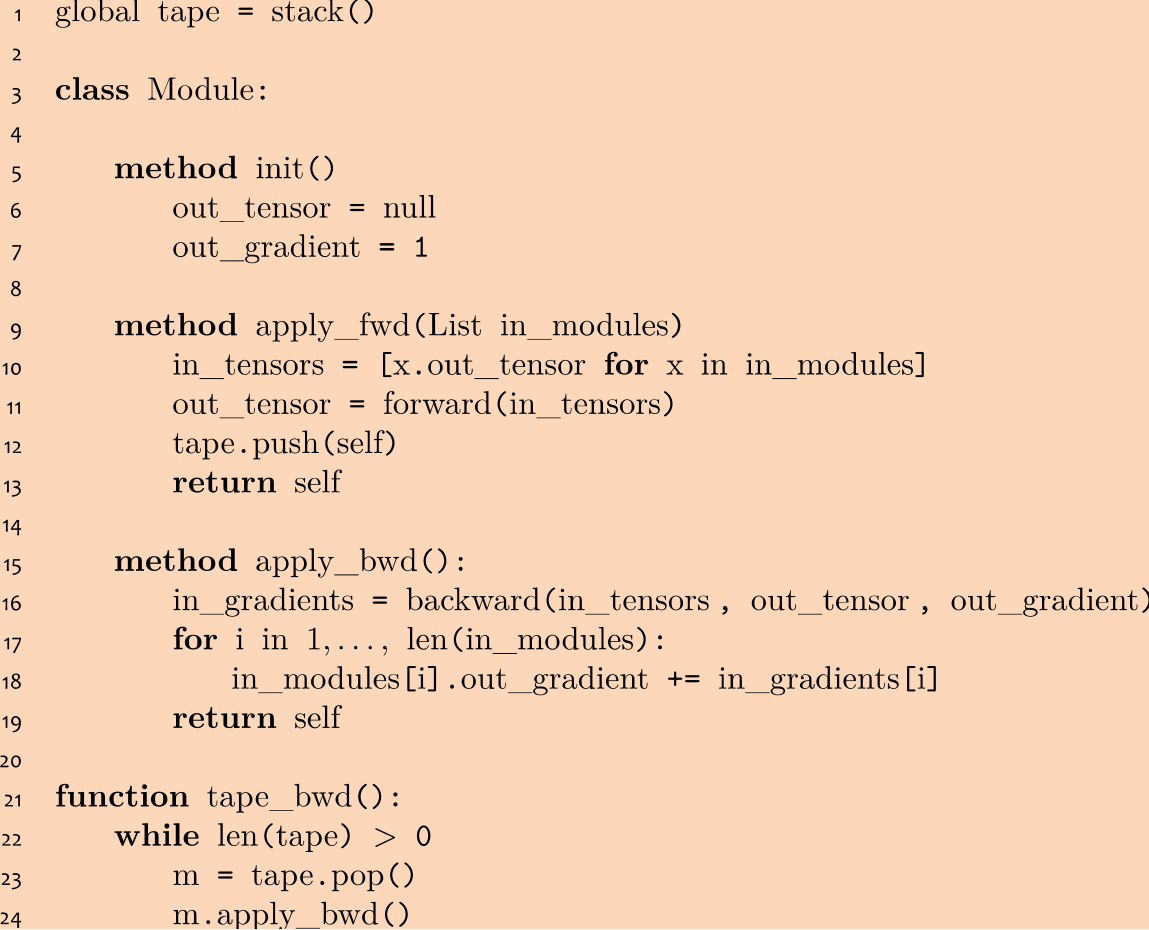
\includegraphics[scale=0.6]{figs/autodiff.png}
\end{figure}

\textbf{Select one:} This is a code snippet from \href{https://www.cs.cmu.edu/~mgormley/courses/10601//slides/lecture19-autodiff-icl.pdf#page=47}{lecture 19 slide 47}. In the context of the \texttt{method apply\_fwd()} inside the \texttt{Module} class, what is the primary role of the \texttt{tape.push(self)} command that pushes the module onto the tape?

    \begin{list}{}
    % YOUR ANSWER
    % Change \emptycircle to \filledcircle for the appropriate selection/selections
        \item 
            \filledcircle
            % \filledcircle
            It records the current module onto the stack along with its parameters and tensors to ensure that the output tensor is saved for the backward pass.
        \item 
            \emptycircle 
            % \filledcircle
            It pushes the current computation's gradient onto the stack for immediate use in the forward pass.

        \item 
            \emptycircle
            % \filledcircle
            It duplicates the module to allow for parallel computations in subsequent layers of the neural network.
 
        \item 
            \emptycircle
            % \filledcircle
            It activates the module for the forward pass, making it the only active computation in the network.
    \end{list}
    

\clearpage
\part[2]  
\textbf{True or False:} We can replace a stack with a queue in Module-based AutoDiff without increasing the runtime of the algorithm. Explain your reasoning in no more than 2 sentences in the box below.
    \begin{list}{}
    % YOUR ANSWER
    % Change \emptycircle to \filledcircle for the appropriate selection/selections
        \item 
            \emptycircle
            % \filledcircle
            True 
        \item 
            \filledcircle 
            % \filledcircle
            False 
    \end{list}

\begin{your_solution}[height=3cm, width=\textwidth]
	\small
	The stack is used to store the order of the operations performed in forward pass, operating in LIFO, Last In First Out, so as to provide the reverse topological order when doing the backward pass. However, a queue operates in FIFO, First In First Out, which does not align with the required reverse ordering execution in backward pass, so replacing the stack with a queue would need extra complexity and increase the runtime to compute the reverse order.
\end{your_solution}

% (Just kidding. We would never replace Neural the Narwhal!)

\part 
Consider a Transformer model employing a multi-headed self-attention mechanism. Suppose the input consists of a sequence of $T$ tokens, each token represented by a $d_{\text{model}}$-dimensional embedding vector. This model utilizes $H$ attention heads. During the attention process, each head generates keys, queries, and values from the input embeddings. The dimensionality of the key and query vectors is $d_k$ for each head, and the attention function produces an output vector of dimension $d_v$ for each token and head.

\begin{subparts}
\subpart[1] Which of the following represents the dimension of the key tensor for a single attention head?

    \begin{list}{}
    % YOUR ANSWER
    % Change \emptycircle to \filledcircle for the appropriate selection/selections
        \item 
            \emptycircle
            % \filledcircle
            $T \times d_v$
        \item 
            \emptycircle 
            % \filledcircle
            $H \times d_k \times d_{\text{model}}$
        \item 
            \filledcircle 
            % \filledcircle
            $T \times d_k$
        \item 
            \emptycircle 
            % \filledcircle
            $T \times d_{\text{model}} \times d_k$
    \end{list}


\subpart[1]  Which of the following represents the dimension of the output tensor of the multi-headed attention before any final linear transformation?

    \begin{list}{}
    % YOUR ANSWER
    % Change \emptycircle to \filledcircle for the appropriate selection/selections
        \item 
            \emptycircle
            % \filledcircle
            $T \times H \times d_k$
        \item 
            \filledcircle 
            % \filledcircle
            $T \times H \times d_v$
        \item 
            \emptycircle 
            % \filledcircle
            $T \times d_{\text{model}}$
        \item 
            \emptycircle 
            % \filledcircle
            $H \times d_k \times d_v$
    \end{list}


\end{subparts}
\end{parts}
    \newpage
\sectionquestion{Empirical Questions}
\label{sec:empirical}

The following questions should be completed as you work through the programming part of this assignment. \textbf{Please ensure that all plots are computer-generated}. For all questions, unless otherwise specified, set \texttt{embed\_dim}, \texttt{hidden\_dim}, and \texttt{batch\_size} to be $128$, \texttt{num\_sequences} to 50,000, and \texttt{dk}, \texttt{dv} to $128$. Upload \texttt{colab\_notebook.ipynb} to Google drive to make running the empirical questions easier. Please use \href{https://drive.google.com/file/d/1mECKLG3NWH9uwFgAYRIdAKrABbTGkbVq/view?usp=sharing}{THIS DATA} for the empirical sections.

\begin{parts}

\part[4] First, we will experiment with changing the size / number of parameters in the model.

Generate two plots, one with the training loss and the other with the validation loss. The y-axis should have the loss value and the x-axis should have the number of sequences utilized for training so far. Each of the two plots should have four lines:
\begin{itemize}
    \item the training/validation loss using \texttt{embed\_dim} = \texttt{hidden\_dim} = $64$,
    \item the training/validation loss using \texttt{embed\_dim} = \texttt{hidden\_dim} = $128$,
    \item the training/validation loss using \texttt{embed\_dim} = \texttt{hidden\_dim} = $256$,
    \item the training/validation loss using \texttt{embed\_dim} = \texttt{hidden\_dim} = $512$,
\end{itemize}
Please \emph{include a legend} that clearly indicates which curve corresponds to which embedding and hidden dimensionalities and \emph{please title the plot} denoting whether it is training or validation loss accordingly

{[}Total expected runtime on Colab T4: 15 minutes{]}

\begin{your_solution}[height=7cm]
    % YOUR TABLE HERE
	\begin{minipage}{0.48\linewidth}
	\centering
	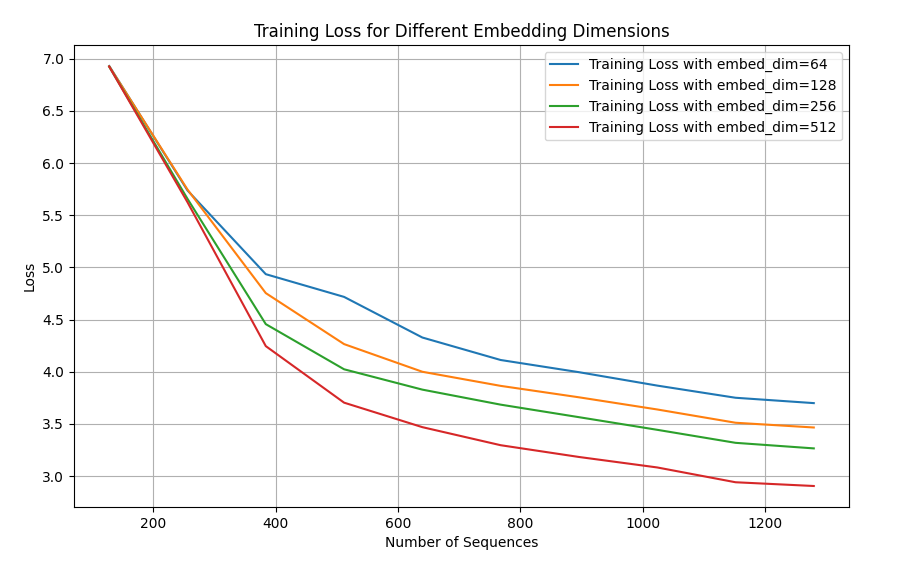
\includegraphics[width=\linewidth]{../handout/Q5_1_training.png}
	\refstepcounter{figure} \\ % Increment the figure counter
	{\tiny \textbf{Figure \thefigure:} Training Loss vs Number of Sequences}  % Manually add a caption/title
	\label{fig:Q5_1_training}         % Label for referencing	
	\end{minipage}
	\hfill
	\begin{minipage}{0.48\linewidth}
	\centering
	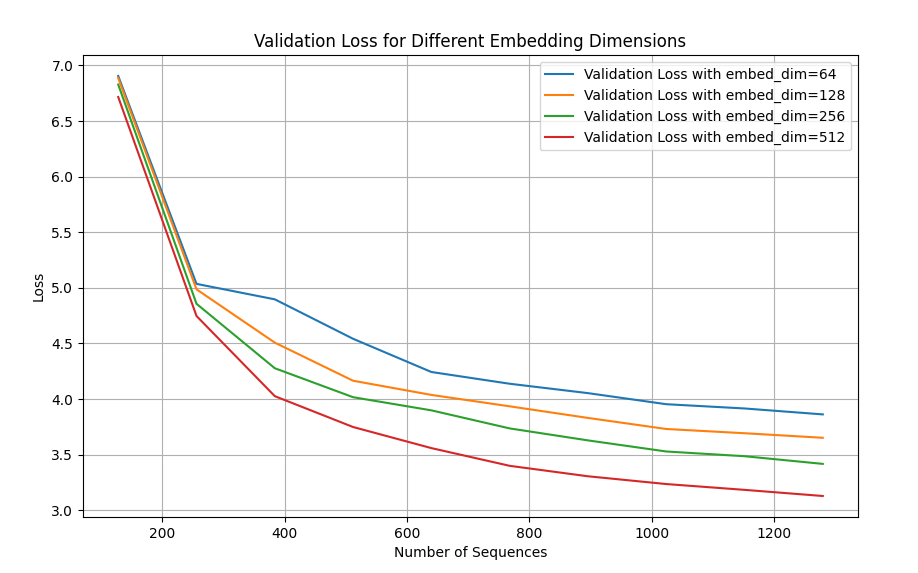
\includegraphics[width=\linewidth]{../handout/Q5_1_validation.png}
	\refstepcounter{figure} \\ % Increment the figure counter
	{\tiny \textbf{Figure \thefigure:} Validation Loss vs Number of Sequences} % Manually add a caption/title
	\label{fig:Q5_1_validation}         % Label for referencing
	\end{minipage}    
\end{your_solution}

\clearpage

\part For this part, we will be experimenting the batch size and observing its impact on both performance during training and validation as well as speed.

\begin{subparts}
    \subpart[4] Generate two plots, one with the training loss and the other with the validation loss. The y-axis should have the loss value and the x-axis should have the number of sequences utilized for training so far. Each of the two plots should have four lines:
    \begin{itemize}
        \item the training/validation loss using \texttt{batch\_size} = $32$,
        \item the training/validation loss using \texttt{batch\_size} = $64$,
        \item the training/validation loss using \texttt{batch\_size} = $128$,
        \item the training/validation loss using \texttt{batch\_size} = $256$,
    \end{itemize}
    
    Please \emph{include a legend} that clearly indicates which curve corresponds to which batch size and \emph{please title the plot} denoting whether it is training or validation loss accordingly.

    {[}Total expected runtime on Colab T4: 20 minutes{]}
    
    \begin{your_solution}[height=7cm]
        % YOUR TABLE HERE
	\begin{minipage}{0.48\linewidth}
	\centering
	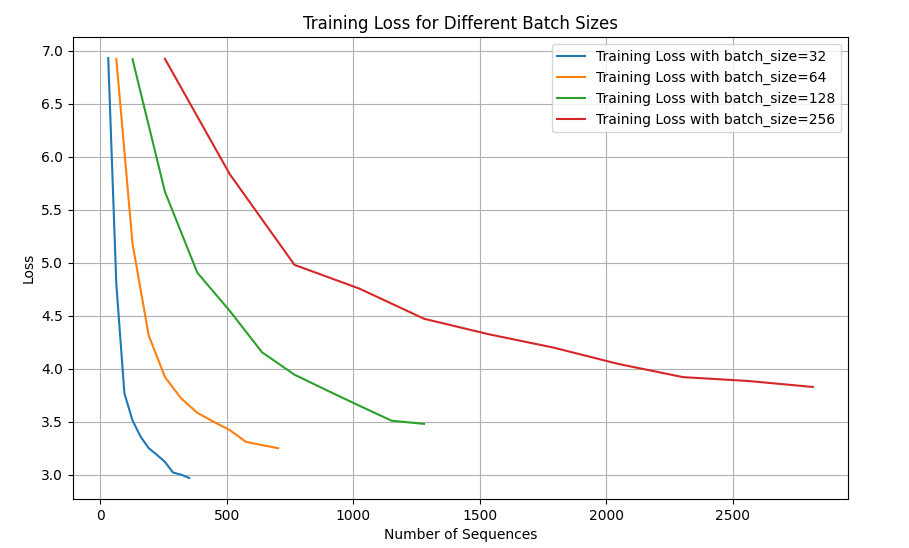
\includegraphics[width=\linewidth]{../handout/Q5_2_training.png}
	\refstepcounter{figure} \\ % Increment the figure counter
	{\tiny \textbf{Figure \thefigure:} Training Loss vs Number of Sequences}  % Manually add a caption/title
	\label{fig:Q5_2_training}         % Label for referencing	
	\end{minipage}
\hfill
	\begin{minipage}{0.48\linewidth}
	\centering
	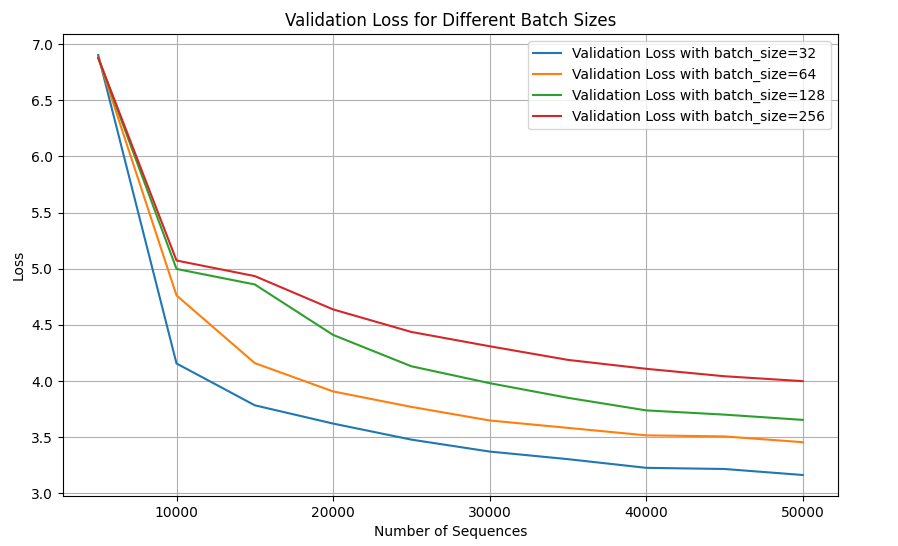
\includegraphics[width=\linewidth]{../handout/Q5_2_validation.png}
	\refstepcounter{figure} \\ % Increment the figure counter
	{\tiny \textbf{Figure \thefigure:} Validation Loss vs Number of Sequences} % Manually add a caption/title
	\label{fig:Q5_2_validation}         % Label for referencing
	\end{minipage}        
    \end{your_solution}
    
    \subpart[2] Report the total time taken for each of the batch sizes from the previous part (a) in the form of a table. The table contains four rows, one each for \texttt{batch\_size} $32$, $64$, $128$, and $256$.
    
    \begin{center}
        \begin{tabular}{c|c}
            % YOUR ANSWER
            \toprule
            {\bf Batch Size}   & {\bf Time (sec)}  \\
            \midrule
            32 & 241.7877  \\
            64 & 124.2302  \\
            128 & 61.0216  \\
            256 & 39.6777  \\
            \bottomrule
        \end{tabular}
    \end{center}
    
    
    \clearpage
    
    \subpart[2]
    Provide a short answer describing the tradeoff between batch size and training speed/performance based on your observations from parts (a) and (b). \\
    \begin{your_solution}[height=4cm]
    	\small
    	Smaller batch sizes lead to longer training time because the model process fewer samples per step, increasing the number of iterations during an epoch. However, smaller batch size brings better performance, lower loss, as more noise in the process of optimization provides more opportunity to escape local minimum.
    	On the other hand, larger batch sizes has much fewer training time because it processes more data at once to further utilize the data parallelism. However, the smoother updated gradients, with less noise, could have a problem of having less opportunity to escape poor local minimum, resulting in worse performance, higher loss, during an epoch.
    \end{your_solution}
\end{subparts}


\part[4] For this question, we will experiment with the number of sequences seen during training and the effects on performance.
    
    Generate two plots, one for training loss and the other for the validation loss. The x-axis would have the \texttt{num\_sequences} and y-axis would contain the \emph{final} training/validation losses. Plot the final training/validation losses for \texttt{num\_sequences}=$10000$, $20000$, $50000$, and $100000$. Unlike previous questions, there will just be a single line in each plot.

    {[}Total expected runtime on Colab T4: 15 minutes{]}
    
    \begin{your_solution}[height=7cm]
        % YOUR PLOT HERE
	\begin{minipage}{0.48\linewidth}
	\centering
	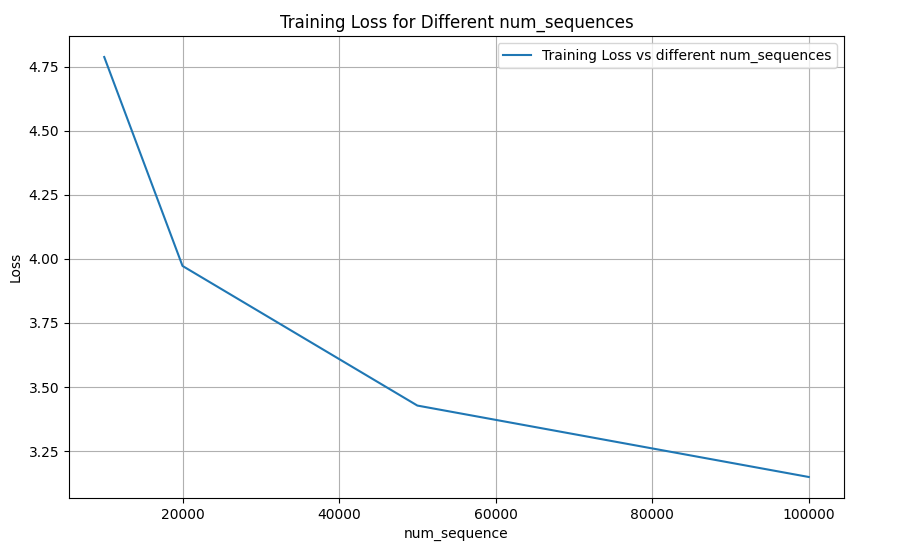
\includegraphics[width=\linewidth]{../handout/Q5_3_training.png}
	\refstepcounter{figure} \\ % Increment the figure counter
	{\tiny \textbf{Figure \thefigure:} Training Loss vs num\_sequences}  % Manually add a caption/title
	\label{fig:Q5_3_training}         % Label for referencing	
	\end{minipage}
	\hfill
	\begin{minipage}{0.48\linewidth}
	\centering
	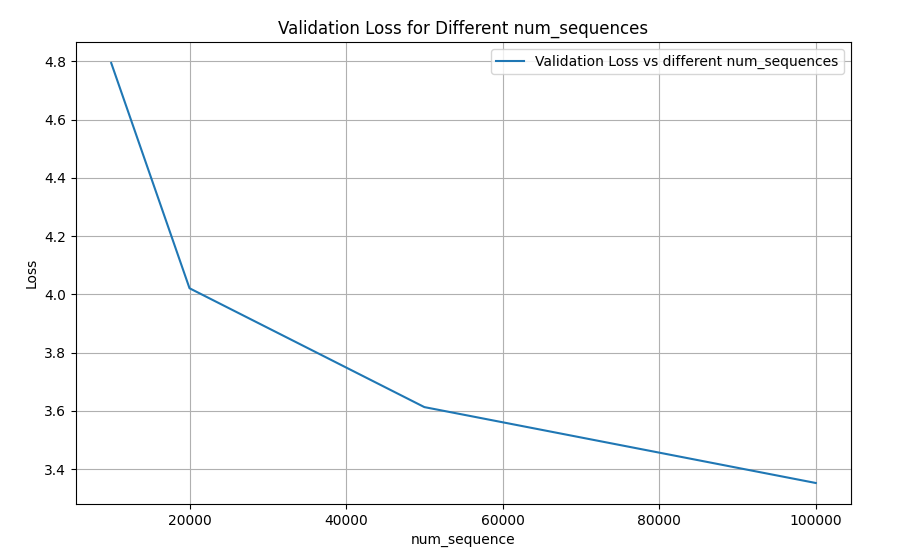
\includegraphics[width=\linewidth]{../handout/Q5_3_validation.png}
	\refstepcounter{figure} \\ % Increment the figure counter
	{\tiny \textbf{Figure \thefigure:} Validation Loss vs num\_sequences} % Manually add a caption/title
	\label{fig:Q5_3_validation}         % Label for referencing
	\end{minipage}        
    \end{your_solution}



\part Finally, we will train a model on significantly more sequences and sample generations at different temperature settings to get very compelling variations of a short story.

\begin{subparts}
    \subpart[3] Fill in the table below with the final train and validation loss, and total running time of the model using the following hyperparameter setting and train the model:
    \begin{itemize}
        \item \texttt{num\_sequences} = $250000$,
        \item \texttt{batch\_size} = $128$,
        \item \texttt{embed\_dim} = \texttt{hidden\_dim} = $512$,
        \item \texttt{key, value dimensions} = 256,
    \end{itemize} 

    {[}Total expected runtime on Colab T4: 30 minutes{]} \\
    
    \begin{center}
        \begin{tabular}{c|c|c}
            % YOUR ANSWER
            \toprule
            {\bf Train Loss}   & {\bf Validation Loss} & {\bf Time (sec)} \\
            \midrule
               2.032871 & 2.285386  &  777.4245 \\
            \bottomrule
        \end{tabular}
    \end{center} 
    


    \subpart[3] Sample three different generations from the above model and report your favorite sample for each value of \texttt{temperature} in the set $\{0, 0.3, 0.8\}$. Using the \texttt{complete} method provided in the starter code, generate completions for the prompt ``Once upon a time there was a''. Include each of the completions below. 

    HINT: Use \texttt{torch.load()} to load the saved model after training is complete to avoid having to re-train the model for each generation.
    
    \begin{your_solution}[title=\texttt{Temperature = 0}, height=3cm]
        % YOUR ANSWER
        \small
        Test prefix: Once upon a time there was a \\
        Test output: footh nose. It was a footh nose. It was a footh nose. It was a footh nose. It was a footh nose. It was a footh nose. It was a footh nose. It was a footh nose. One no
    \end{your_solution}
    
    \begin{your_solution}[title=\texttt{Temperature = 0.3}, height=3cm]
        % YOUR ANSWER
        \small
		Test prefix: Once upon a time there was a \\
		Test output: little girl called Mary. She was three years old and loved to swim in the sand. One day, she found a sandwich in the sandwich and it was very dirty. She wanted to swim in the sandwich. She was very happy and she wanted to swim and swimming in the sandwich. She asked her mom, "Can I swimsee        
    \end{your_solution}
    
    \begin{your_solution}[title=\texttt{Temperature = 0.8}, height=3cm]
        % YOUR ANSWER
        \small
		Test prefix: Once upon a time there was a \\
		Test output: little boy called John. He had a special turtle. He liked to run and jump and jump around the turtle, and going the turtle of the castle. He was very scared and tried to sleep. He didn't want to, but he was just a bit sad. He wanted to pick on the turtle of the turtles so he had made a mess. The turtle was so happy that he knew it was ia not
    \end{your_solution}


    \clearpage
    \subpart[1]Describe the trend in the generated completions as \texttt{temperature} increases. Which value generated the ``best'' completions in your opinion?

    \begin{your_solution}[height=4cm]
        % YOUR ANSWER
        \small
        As the temperature increases, the content of the generated text becomes more and more random and various, and at the meanwhile the coherence between sentences becomes lesser and lesser. When temperature = 0, the model just repeats the same, most probable, words over and over. When temerature = 0.3, the output is more various, including some randomness and creativity. When temperature = 0.8, the output shows even more diverse contents and creativity, but lacks of coherence. In my opinion, temperature with 0.3 generates the best output that retains and balances between creativity and coherence.
    \end{your_solution}
\end{subparts}

\end{parts}
    \newpage
    \end{questions}
\newpage
\section{Collaboration Questions}
After you have completed all other components of this assignment, report your answers to these questions regarding the collaboration policy. Details of the policy can be found \href{http://www.cs.cmu.edu/~mgormley/courses/10601/syllabus.html}{here}.
\begin{enumerate}
    \item Did you receive any help whatsoever from anyone in solving this assignment? If so, include full details.
    \item Did you give any help whatsoever to anyone in solving this assignment? If so, include full details.
    \item Did you find or come across code that implements any part of this assignment? If so, include full details.
\end{enumerate}

\begin{your_solution}[height=6cm]
% YOUR ANSWER 
\begin{enumerate}
    \item No.
	\item No.
	\item No.
\end{enumerate}	
\end{your_solution}

\newpage
\section{Programming: Language Modeling (55 points)}
\label{programming}

Large language models (LLMs) like ChatGPT, Gemini, and LLaMA have achieved unprecedented levels of success (and hype) over the past few years. In this section, you will become familiar with the building blocks of these models by implementing your very own Recurrent Neural Network \textsc{l}LM\footnote{\textit{Little} lanugage model} with self-attention.

You will be building your model using PyTorch, a widely-used open source deep learning library. \textcolor{red}{In this homework, you can and should call any built-in PyTorch module (e.g., \texttt{nn.Linear}) \textit{except} \texttt{nn.RNNCell}, \texttt{nn.RNN} and \texttt{nn.MultiheadAttention} or any “functional equivalents” of these.}



\subsection{Libraries (IMPORTANT)}

We will be using the following libraries \textit{only} for this assignment. Make sure that the versions in your local environment match the ones listed here.

\begin{lstlisting}
torch==2.2.2
transformers==4.40.1
numpy==1.23.0
\end{lstlisting}

You should not use \texttt{transformers} for anything other than loading in the tokenizer. In the handout, we have given a file called requirements.txt. In your environment, please run \begin{lstlisting}
pip install -r requirements.txt
    
\end{lstlisting}

\subsection{The Task}\label{task}

Language modeling is the task of assigning probabilities to texts (i.e. sequences of tokens). Language modeling is most commonly done with \textit{autoregressive} models, which use the chain rule of probability to decompose the probability of a text $\xv = [ x_1, x_2, \ldots, x_n ]$ as follows:
\begin{align*}
    P(\xv) = P(x_1) P(x_2 | x_1) P(x_3 | x_1, x_2) \cdots P(x_n | x_1,\ldots,x_{n-1})
\end{align*}
In other words, an autoregressive language model is tasked with predicting the conditional probability of the next token given all the tokens that came before it, $P(x_{t+1} | x_1,\ldots,y_{x})$. In Section 5.5, we will see how these conditional probabilities will be computed by your RNN language model.


\subsection{The Dataset}\label{dataset}
We will be training RNN-LMs on the \href{https://huggingface.co/datasets/roneneldan/TinyStories}{TinyStories} dataset, a collection of 2 million short stories with simple vocabularies generated by GPT-3.5 and GPT-4. Small language models trained on this data have been shown to have a high level of English fluency, strong storytelling abilities, and reasoning capabilities. We will be using a subset of this data. The dataset has already been processed for you in the SentenceDataset class, and batched in the dataloader, so you don't need to worry about loading the data. We do provide a sample of what the data looks like in the \texttt{untokenized\_train\_stories.json} and \texttt{untokenized\_valid\_stories.json}. Feel free to see what the stories look like.


\subsubsection{Tokenization}

By their nature, ML models are unable to directly operate on text strings. As such, we have to first \textit{tokenize} text into sequences of tokens by assigning numerical values to substrings (i.e. words, characters, punctuation, even whitespace). 
In this particular homework, we will be using \textit{subword tokenization}, the kind of tokenization usually used by state-of-the-art language models like GPT-4 and LLaMA. This flavor of tokenization splits text up into subwords, which may be either full words or parts of words (for example, the ``-ed'' past tense suffix). 

In the \texttt{my\_tokenizer} directory of the handout, we have provided you with a pretrained tokenizer for the TinyStories dataset, which can be loaded using the \texttt{transformers} library:

\begin{lstlisting}
>>> from transformers import AutoTokenizer
>>> tokenizer = AutoTokenizer.from_pretrained("my_tokenizer")
>>> tokenizer.encode("We like ML.")
[360, 192, 110, 1010, 1017, 103, 1]
>>> tokenizer.decode([360, 192, 110, 1010, 1017, 103, 1])
'We like ML.</s>'
\end{lstlisting}

Note that the training and validation data has already been tokenized for you. However, if you would like to convert tokens back to text, you can use the \texttt{tokenizer.decode} method, as shown above.


\subsection{Required Reading: PyTorch Tutorial}

Before proceeding any further, you must complete the PyTorch Tutorial. Please read the full collection of the Introduction to PyTorch, i.e. Learn the Basics $\|$ Quickstart $\|$ Tensors $\|$ Datasets \& DataLoaders $\|$ Transforms $\|$ Build Model $\|$ Autograd $\|$ Optimization $\|$ Save \& Load Model.    

    \url{https://pytorch.org/tutorials/beginner/basics/intro.html}
    

\subsection{Model Definition}\label{model}
In this homework, you will create a language model that uses an RNN backbone to score and generate text in \texttt{rnn.py} (starter code for this file is provided in the handout).

\begin{figure}[htp]
    \centering
    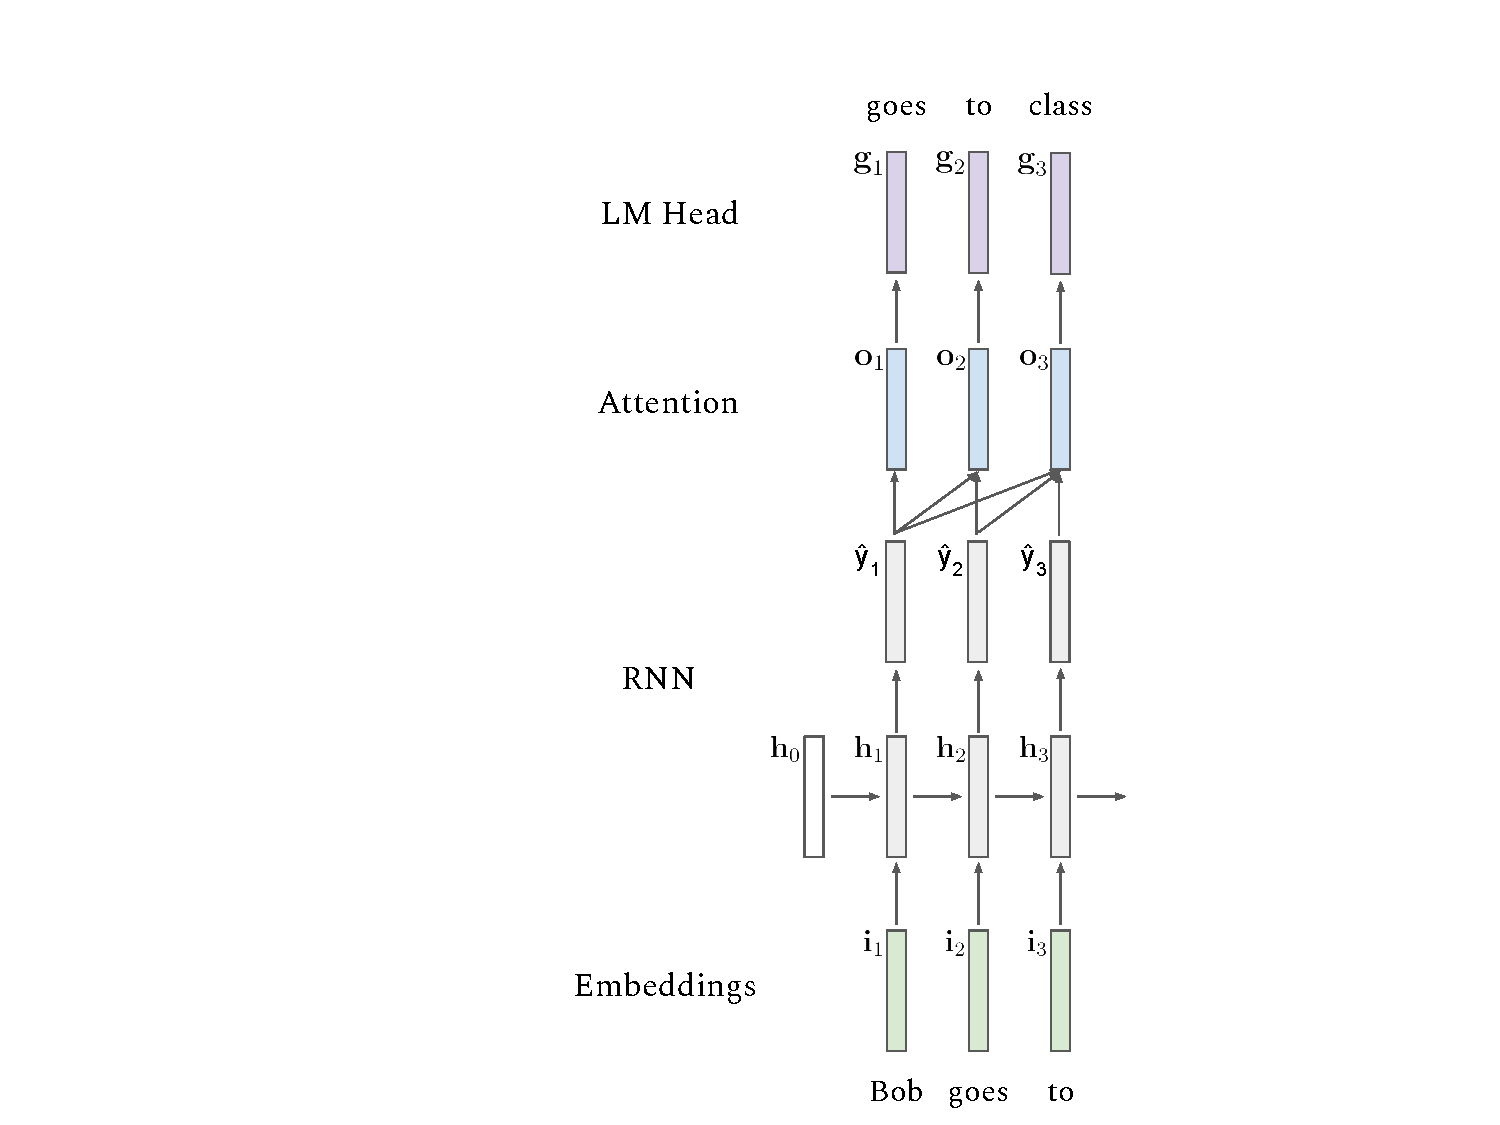
\includegraphics[scale=0.5]{figs/rnn_diagram.pdf}
    \caption{Computation graph of RNN with attention.}
    \label{fig:enter-label}
\end{figure}

\subsubsection{RNN Cell}

This is the building block of the RNN, representing a single RNN step. This class has a single method, \texttt{forward}, which takes in the batched input for the current step $\iv_t$ and the previous hidden state $\hv_{t-1}$ and outputs the next hidden state $\hv_t$. Recall that the hidden state is defined as follows:
\begin{align*}
    \hv_t = \phi( \Wv_\text{i2h} \iv_t + \Wv_\text{h2h} \hv_{t-1} )
\end{align*}
where $\phi$ is an activation function, either ReLU or $\tanh$ in this assignment.
\textbf{Hint:} Here (and in the rest of the model definition, including in say Section 7.5.1), matrix products like $\Wv_\text{i2h} \iv_t$ correspond to \texttt{nn.Linear} layers in PyTorch.

\subsubsection{Self-Attention}

In \lstinline{SelfAttention} you will implement scaled dot product attention. Both methods in this class will take in a sequence of vectors up to the current timestep $t$, $[\hat{\yv_1}, \ldots, \hat{\yv_t}]$. Note that the computation is batched, but for the sake of simplicity we write the equations below for a sample. In this case, the query, keys, and values are defined as follows.
\begin{align*}
\qv_t = \Wv_q \hat{\yv_t} \\
\kv_t = \Wv_k \hat{\yv_t}\\
\vv_t = \Wv_v \hat{\yv_t}
\end{align*}
Then, the output of the attention module will be the attention vector for the current timestep, $\av_t$, computed by a weighted average of the values. Note that we use scaled dot-product attention (as proposed in the original transformers paper), which divides the dot product of the key and query vectors by the dimension of the keys, $D_\text{key}$.
\begin{align*}
    \sv &= \bigg[ \frac{\kv_1 \cdot \qv_t}{\sqrt{D_\text{key}}}, \frac{\kv_2 \cdot \qv_t}{\sqrt{D_\text{key}}}, \ldots, \frac{\kv_t \cdot \qv_t}{\sqrt{D_\text{key}}}, \bigg]^T \tag{Attention Scores} \\
    \wv &= \text{Softmax}(\sv) \tag{Attention Weights} \\
    \av_t &= \Wv_o \left(\sum_{n=1}^t w_n \vv_n\right)
\end{align*}

For this class, you will implement two functions:

\texttt{step()}: Given the predictions for all timesteps, compute the attention for just the prediction at the current time step, $\hat{\yv_t}$, using the above equations. Be very careful about the dimensions that you transpose in order to calculate the attention scores correctly for $\sv$. At the end, we apply an additional transform to get our output $\ov_t$.

\texttt{forward()}: Compute the attention for predictions across all timesteps, $[\hat{\yv_1}, \ldots, \hat{\yv_t}]$. It is recommended to use the previously implemented \texttt{step()} function to calculate the outputs iteratively over the timesteps. Then, concatenate all of the outputs along the sequence length (number timesteps $t$) dimension to get output states $[\ov_1, \ldots, \ov_t]$

\subsubsection{RNN}

This class represents the entire RNN and processes an entire batched sequence $[\iv_1, \iv_2, \ldots \iv_T]$. Note the distinction between this class and RNNCell: RNNCell's \texttt{forward} method runs a single step of the input sequence, while RNN's \texttt{forward} runs for all steps of the input sequence. Hence, this class contains (up to) two modules, (1) the RNN cell and (2) Linear layer to project \texttt{hidden\_size} to \texttt{hidden\_size}. This class has two methods, \texttt{step} and \texttt{forward}.

\texttt{step()}: This method processes a single step of the batched input sequence. Specifically, it takes both in the current input $\iv_t$ and all preceding hidden states $[\hv_1, \ldots \hv_{t-1}]$ and returns both the next hidden state $\hv_t$ and the next output state of the RNN $\hat{\yv_t}$. 

\texttt{forward()}: This method processes an entire batched input sequence $[\iv_1, \iv_2, \ldots \iv_T]$. It should iteratively call \texttt{step} on each vector in the input sequence, along with the appropriate hidden states argument. It should return the hidden states $[\hv_1, \hv_2, \ldots, \hv_T]$ and output states $[\hat{\yv_1}, \hat{\yv_2}, \ldots, \hat{\yv_T}]$ over all steps.


\subsubsection{RNN Language Model}

Now, we can use the RNN backbone we have defined in the previous sections to create our very own \textsc{l}LM. However, we will need to add a couple modules on both ends of the RNN. Before the RNN, we need an embedding layer to convert integer token indices $[x_1, \ldots, x_T]$ to vector embeddings $[\iv_1, \ldots, \iv_T]$ that can be passed into the RNN as inputs. 
\textbf{Hint:} use \texttt{nn.Embedding} for this. 

Then, we declare the RNN module, based on the size of the vector embeddings to the hidden dimension to get all of the output states to be fed at once in the Attention Layer.

Next, initialize a Self Attention layer, with inputs of hidden, key, query dimensions. 

Finally, we will need to add a language modeling head, a linear layer $W_\text{LM}$ that projects the RNN output $\ov_t$ to the next-token logits $\gv_t = W_\text{LM} \ov_t$. These logits are not actually the next-token distribution; rather, they are ``raw scores" that can be fed into a softmax to yield the distribution. Hence, we have that
\begin{align*}
    P(x_{t+1} | x_1, \ldots, x_t) = \text{Softmax}(\gv_t)
\end{align*}

This module has three functions:

\texttt{forward()}: Calls all of the modules in the order as discussed above. To recap, we create embeddings from the input Tensor and then get the hidden states and predictions from the RNN forward. Call Self Attention on these predictions and then apply the LM head. Finally, return the tokens generated from the LM head and the RNN hidden/output states.

\texttt{select\_token()}: This function has been implemented already. It will sample a token from the probability distribution based on the sampling policy. For greedy sampling, we just take the argmax. For temperature sampling, we need to re-compute the probability distribution and randomly sample $1$ token.

\texttt{generate()}: This function has been implemented already. It will call \texttt{select\_token()}, RNN, SelfAttention iteratively until we reach the max number of tokens. Note that the initial call to the model's \texttt{forward()} function computes all of the outputs and hidden states for the prefix string, then calls the \texttt{step()} function for RNN and SelfAttention because generating tokens one-by-one and don't have access to the entire sequences at once anymore.


\subsection{Training and Evaluation}\label{train_and_eval}

Now that you have created a working model, it's time to train and evaluate it! For this section, you will complete two functions: \texttt{train()} and \texttt{validate()}.

\texttt{train()}: This function will train the model, and validate the model every 10\% that we process. The argument \texttt{num\_sequences} specifies how long we train for, for every tenth that we progress we will validate our model. Note that this is a little different from what you are used to, since we are not using epochs as a way to control the training, instead we are controlling it by setting the number of sequences the model will process. This is so that the model can see a more diverse set of sequences as opposed to looping over the same set multiple times.

We will use the same loss function as in HW5, cross entropy loss. Here, the cross entropy is computed between the predicted next-token distribution $P(\hat{y}_{t+1}|y_1, \ldots, y_t)$ and a target one-hot distribution with a 1 at the index corresponding to the true next token $y_{t+1}$. This loss should be computed for each token and then averaged over the sequence. Please see the \texttt{nn.CrossEntropyLoss} PyTorch documentation for instructions on how it should be used to compute the cross entropy loss.

Be careful to correctly shift the target tokens. For instance, the target for the first token is not the first token itself but the second (i.e., the next token). Also, as there is no token after the last token $x_T$, there can be no target for the last step's predicted next-token distribution $P(x_{T+1} | x_1, \ldots, x_T)$. Thus, we can only compute loss for the first $T-1$ tokens in the sequence.

\texttt{validate()}: This function computes the average loss over a validation dataset. This should be implemented nearly the same as the \texttt{train} method, minus the gradient updates to the model.

\subsection{Text Generation}
While we have been training language models to compute probabilities over texts, they are more than probability estimators! Instead of using the next-token distribution to score existing tokens, we can also use it to predict new ones.

Suppose we are given a text prefix consisting of tokens $\xv = [x_1, \ldots, x_m]$. Then when we pass the final token $x_m$ into our language model, we will get next token logits $\gv_m$ which imply a distribution $P(x_{m+1} | x_1, \ldots, x_m)$. In this homework, you will implement two methods of picking a next token $\hat{x}_{m+1}$ using this distribution:

\begin{enumerate}
    \item \textbf{Greedy:} Pick the next token with the highest probability.
    \begin{align*}
        \hat{x}_{m+1} = \argmax_{x_{m+1}} P(x_{m+1} | x_1, \ldots, x_m)
    \end{align*}
    \item \textbf{Temperature Sampling:} Rather than deterministically picking the highest probability next token, we can also randomly sample a next token. However, we don't necessarily have to sample from the next-token distribution $P(x_{m+1} | x_1, \ldots, x_m)$ itself. Instead, we will sample from a slightly different \emph{temperature-adjusted} distribution $Q$:
    \begin{align*}
        Q(x_{m+1} | x_1, \ldots, x_m) &= \text{Softmax}(\gv_m / \tau) \\
        \hat{x}_{m+1} &\sim Q(x_{m+1} | x_1, \ldots, x_m)
    \end{align*}
    where $\gv_m$ refers to the next-token logits (as defined in 5.5.4) and $\tau$ is a sampling parameter referred to as the ``temperature''. The value of $\tau$ affects how ``random'' the samples are. Increasing the value of $\tau$ increases ``randomness," while setting $\tau = 0$ recovers greedy decoding.
\end{enumerate}
After picking a token, this token can be fed back into the language model (i.e., get its embedding, feed that into the next step of the RNN, etc...) to yield another next-token distribution. This process can be repeated until some stopping criterion is met.



\subsection{Command Line Arguments}\label{command}
The autograder runs and evaluates the output from the files generated, using the following command:

\begin{tabbing}
\=\texttt{\$ \textbf{python3} rnn.\textbf{py} [args\dots]}\\
\end{tabbing}
    
Where \texttt{[args\dots]} is a placeholder for command-line arguments: \texttt{<train\_data>} \texttt{<val\_data>}

Additional hyper-parameters for the model utilize ``double dashes''. You should experiment with these arguments to improve the performance of the model in the empirical section. \texttt{<--embed\_dim>} \\ \texttt{<--hidden\_dim>}, \texttt{<--dk>}, \texttt{<--dv>}, \texttt{<--num\_sequences>}, \texttt{<--batch\textunderscore size>}

These arguments are described below:
\begin{enumerate}
    \item \texttt{<--train\_data>}: string path to the training input \texttt{.txt} file 
    % (see Section~\ref{dataset})
    \item \texttt{<--val\_data>}: string path to the validation input \texttt{.txt} file 
    \item \texttt{<--metrics\_out>}: string path to the ouptput \texttt{.txt} file to write the final train and validation loss to
    \item \texttt{<--train\_losses\_out>}: string path to the output \texttt{.txt} file to write the training losses to
    \item \texttt{<--val\_losses\_out>}: string path to the output \texttt{.txt} file to write the validation losses to
     \item \texttt{<--embed\_dim>} positive integer specifying the size of the sentence embedding vector \textbf{(hyper-parameter)}
    \item \texttt{<--hidden\_dim>} positive integer specifying the number of hidden units to use in the model's hidden layer \textbf{(hyper-parameter)}
    \item \texttt{<--dk>}: integer specifying size of the keys in self attention \textbf{(hyper-parameter)}
    \item \texttt{<--dv>}: integer specifying size of the values in self attention \textbf{(hyper-parameter)}
    \item \texttt{<--num\_sequences>} positive integer specifying how many sequences to process \textbf{(hyper-parameter)}
    \item \texttt{<--batch\textunderscore size>} batch size of the experiment \textbf{(hyper-parameter)}
\end{enumerate}

Below is an example command to run

\begin{lstlisting}
python3 rnn.py --train_data data/train_stories.json \
--val_data data/valid_stories.json \
--train_losses_out train_losses.txt \ 
--val_losses_out val_losses.txt \
--metrics_out metrics.txt \
--embed_dim 64 --hidden_dim 128 \
--dk 32 --dv 32 --num_sequences 128 --batch_size 1 
\end{lstlisting}
\vspace{0.2 in}

\subsection{Outputs and Tests} 
Your code should write out a single output file (path given by the \texttt{--metrics\textunderscore out} flag) containing the train and validation losses per epoch. Metrics writing is already taken care of for you in the starter code.

To help you debug your code, we’ve included a test file in your handout, \texttt{test\textunderscore rnn.py}. This is a nonex-haustive set of tests which are meant to help you make sure your implementation is correct. Passing these tests does not guarantee a full score in your Gradescope submission, but it will help you identify functions which have errors. Do not edit these tests as we will not be able to guarantee correctness if you modify these tests. To run the test, run the following command line:
\begin{lstlisting}[language=Shell]
python3 test_rnn.py
\end{lstlisting}

In addition, for debugging purposes, we have included ``tiny" versions of the train and validation datasets and a file \texttt{tiny\_metrics.txt} which contains metrics for the following command:
\begin{lstlisting}
python3 rnn.py --train_data data/tiny_train_stories.json \
--val_data data/tiny_valid_stories.json \
--train_losses_out tiny_train_losses.txt \ 
--val_losses_out tiny_val_losses.txt \
--metrics_out tiny_metrics.txt \
--embed_dim 64 --hidden_dim 128 \
--dk 32 --dv 32 --num_sequences 128 --batch_size 1 
\end{lstlisting}

Your metrics should match these to at least 3-4 decimal places. There may be some more deviation if you run your code locally/on Colab with a GPU, but all Gradescope submissions will be run on CPU so this should not be an issue.

\subsection{Gradescope Submission}

You should submit your \texttt{rnn.py} (\textbf{Note}: you must submit a \texttt{.py} file, \texttt{.ipynb} files will not be processed correctly). \textbf{Any other files will be deleted.} Please do not use other file names. This will cause problems for the autograder to correctly detect and run your code.

% Some additional tips: 
% Make sure to read the autograder output carefully. The autograder for Gradescope prints out some additional 
% information about the tests that it ran. For this programming assignment we’ve specially designed some buggy implementations that you might implement and will try our best to detect those and give you some more useful feedback in Gradescope’s autograder. Make wise use of autograder’s output for debugging your code.

\textit{Note:} For this assignment, you have 10 submissions to Gradescope before the deadline, but only your last submission will be graded.
\end{document}